\chapter{Technologische Randvoorwaarden}
\chplab{technology}
\chapterquote{De enige limiet aan de realisatie van de toekomst is ons twijfelen van vandaag.}{Franklin D. Roosevelt, Amerikaans staatsman en president (26e) (1882-1945)}
\begin{chapterintro}
Tot nu toe hebben we altijd abstractie gemaakt van de werkelijkheid. We hebben in \chpref{basis} poorten ge\"introduceerd, maar hebben altijd abstractie gemaakt van de concrete werking van deze poorten. Aan de hand van het lichtmodel konden we \'e\'en en ander verklaren, maar deze schakelaars moesten manueel geschakeld worden. In dit hoofdstuk zullen we een manier zien hoe we poorten kunnen implementeren, en een $0$ en $1$ kunnen voorstellen die gebruik maakt van elektronica. Dit is uiteraard slechts \'e\'en manier. Naast het implementeren van poorten stuiten we vaak op allerhande fysische problemen. Dit hoofdstuk geeft een overzicht van de verschillende aspecten die we in de gaten moeten houden bij het ontwerpen van een elektronische schakeling. Verder biedt het een overzicht van manieren om een digitale schakeling te realiseren. Tot slot bekijken we de ontwikkeling van digitale schakeling met een CAD tool.
\end{chapterintro}
\minitoc[n]
\section{Logische waarden voorstellen}
\seclab{logischeWaarden}
Alvorens we enige schakeling kunnen implementeren moeten we een conventie afspreken hoe we een $0$ en $1$ voorstellen. Deze logische waarden moeten we voorstellen door twee fysische waarden. Deze fysische waarden noemen we ``\gtermen{High}{De fysische waarde die we associ\"eren met een $1$ of $0$ (bij negatieve logica); bij een implementatie met elektronica is dat meestal een hoge spanning.}'' en ``\gtermen{Low}{De fysische waarde die we associ\"eren met een $0$ of een $1$ (bij negatieve logica); bij een implementatie met elektronica is dat meestal een lage spanning.}''. In de elektronica kiezen we meestal als fysische grootheid de spanning. De referentie-spanningen noteren we dan respectievelijk als $V_{\mbox{\tiny H}}$ en $V_{\mbox{\tiny L}}$.

\paragraph{}
Omdat het moeilijk is om een constante spanning aan de uitgangen aan te leggen, kiezen we niet voor \'e\'en spanning, maar defini\"eren we een bereik rond $V_{\mbox{\tiny H}}$ en $V_{\mbox{\tiny L}}$. Immers is het systeem niet volledig deterministisch, en er kunnen bijgevolg kleine variaties in de spanningen optreden. Daarnaast hebben we ook nog allerhande omgevingsparameters zoals de temperatuur, waardoor deze spanning sowieso enigszins zal afwijken. Tussen het bereik van $V_{\mbox{\tiny H}}$ en $V_{\mbox{\tiny L}}$ defini\"eren we ook nog een zone waar het niet duidelijk is of er een $1$ of $0$ op staat. Dit laat ons toe om fouten te detecteren. Indien de spanning immers dicht bij het midden ligt, is de kans op een foute interpretatie groot. Met een detectiesysteem zouden we dan bijvoorbeeld kunnen vragen om de bit opnieuw uit te sturen. We defini\"eren het bereik van $V_{\mbox{\tiny H}}$ als $\left[V_{\mbox{\tiny IH}},V_{\mbox{\tiny DD}}\right]$, dat van $V_{\mbox{\tiny L}}$ als $\left[V_{\mbox{\tiny SS}},V_{\mbox{\tiny IL}}\right]$. \figref{potentialRange} toont schematisch het bereik van deze waarden. Overigens hebben $V_{\mbox{\tiny DD}}$ en $V_{\mbox{\tiny SS}}$ nog een andere betekenis bij een circuit: het zijn de spanningen die op de voeding van het elektronische apparaat geplaatst worden. Hierbij staat de S voor ``\gtermen{Source}{Een connectie van een FET transistor.}'' en D voor ``\gtermen{Drain}{Een connectie van een FET transistor.}''.

\begin{figure}[hbt]
\centering
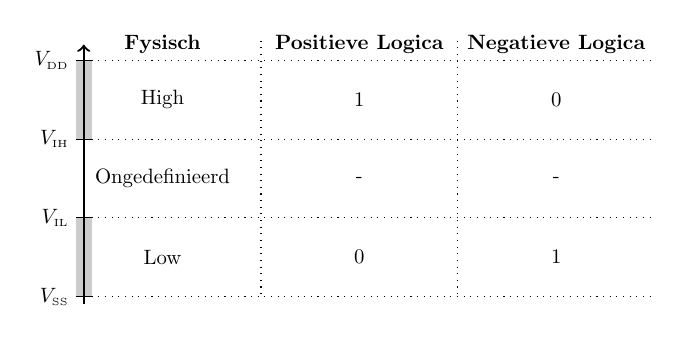
\begin{tikzpicture}
\fill[black!20] (-0.1,0) rectangle (0.1,1);
\fill[black!20] (-0.1,2) rectangle (0.1,3);
\draw[thick,->] (0,-0.1) -- (0,3.2);
\draw (-0.1,0) node[anchor=east,scale=0.75]{$V_{\mbox{\tiny SS}}$} -- (0.1,0);
\draw (-0.1,1) node[anchor=east,scale=0.75]{$V_{\mbox{\tiny IL}}$} -- (0.1,1);
\draw (-0.1,2) node[anchor=east,scale=0.75]{$V_{\mbox{\tiny IH}}$} -- (0.1,2);
\draw (-0.1,3) node[anchor=east,scale=0.75]{$V_{\mbox{\tiny DD}}$} -- (0.1,3);
\draw (1,3) node[scale=0.75,anchor=south]{\bf Fysisch};
\draw (3.5,3) node[scale=0.75,anchor=south]{\bf Positieve Logica};
\draw (6,3) node[scale=0.75,anchor=south]{\bf Negatieve Logica};
\draw (1,2.5) node[scale=0.75]{High};
\draw (1,1.5) node[scale=0.75]{Ongedefinieerd};
\draw (1,0.5) node[scale=0.75]{Low};
\draw (3.5,2.5) node[scale=0.75]{1};
\draw (3.5,1.5) node[scale=0.75]{-};
\draw (3.5,0.5) node[scale=0.75]{0};
\draw (6,2.5) node[scale=0.75]{0};
\draw (6,1.5) node[scale=0.75]{-};
\draw (6,0.5) node[scale=0.75]{1};
\draw[dotted] (2.25,3.25) -- (2.25,0);
\draw[dotted] (4.75,3.25) -- (4.75,0);
\draw[dotted] (0.1,3) -- (7.25,3);
\draw[dotted] (0.1,2) -- (7.25,2);
\draw[dotted] (0.1,1) -- (7.25,1);
\draw[dotted] (0.1,0) -- (7.25,0);
\end{tikzpicture}
\caption{Schematisch bereik van ``High'' en ``Low'' spanning.}
\figlab{potentialRange}
\end{figure}

\paragraph{Negatieve logica}
Het is niet per definitie zo dat $V_{\mbox{\tiny H}}$ geassocieerd wordt met $1$, en $V_{\mbox{\tiny L}}$ met $0$. Dit hangt af van het type logica dat gehanteerd wordt. We onderscheiden twee soorten logica: \gtermen{positieve logica}{Een vorm van implementeren van logica waarbij we een hoge spanning associ\"eren met een $1$ en een lage spanning met een $0$.} en \gtermen{negatieve logica}{Een vorm van implementeren van logica waarbij we een hoge spanning associ\"eren met een $0$ en een lage spanning met een $1$.}. In geval van positieve logica is dit inderdaad het geval. Soms komt het echter voordeliger uit om deze orde om te draaien, in dat geval spreekt men van negatieve logica. Merk op dat bij negatieve logica de poorten fysisch anders ge\"implementeerd moeten worden. Immers kent de fysische poort alleen maar spanningen, en geen $0$ of $1$. De belangrijkste reden om negatieve logica te gebruiken, is dan ook dat de implementatie van een logische functie goedkoper kan zijn in bijvoorbeeld negatieve logica. Bovendien kan men in een circuit op verschillende plaatsen een andere logica gebruiken. Een concreet voorbeeld is de reset-module in veel elektronicasystemen die men vaak in negatieve logica realiseert.

\section{Implementatie van poorten}
\subsection{Schakelaars}
In \chpref{basis} maakten we gebruik van het lichtmodel om poorten te implementeren. Daarbij werd gebruik gemaakt van schakelaars. Ook in de echte implementatie van poorten maakt men gebruik van \gtermen{schakelaars}{Een component waar - afhankelijk van een stuursignaal of toestand - er al dan niet stroom door vloeit.}. Deze schakelaars kunnen door een derde ingang automatisch open en dicht geschakeld worden, deze ingang wordt ook het ``\gtermen{stuursignaal}{Een signaal bij een generische transistor. Het stuursignaal (vaak ``basis'' genoemd) beslist of er stroom tussen de collector en de emitor stroomt.}'' genoemd.

\paragraph{}
Net als de schakelaars in het lichtmodel hebben deze schakelaars twee toestanden: \gtermen{open}{Een toestand bij een schakelaar waarbij er geen stroom door de schakelaar vloeit.} en \gtermen{gesloten}{Een toestand bij een schakelaar waarbij er stroom vloeit door de schakelaar.}. We kunnen dit interpreteren als een elektronische weerstand die respectievelijk een weerstand van $\infty\ \Omega$ en $0\ \Omega$ heeft. \figref{switchNotationSwitch} toont hoe dergelijke schakelaars genoteerd worden. Afhankelijk van hun toestand worden ze bovendien anders genoteerd\footnote{In algemene schemas maken we abstractie van de toestand en is deze niet zichtbaar.}.

\paragraph{}
Zoals eerder gezegd dienen deze automatische schakelaars een stuursignaal te hebben. Op \figref{switchNotationControlledNmos} en \figrefn{switchNotationControlledPmos} staan de schakelaars met stuursignaal. We merken op dat er twee varianten van schakelaars zijn. De ene variant, \gtermen{NMOS}{Een variant van een automatische schakelaar waarbij de schakelaar gesloten is indien het stuursignaal hoog is; en open indien het stuursignaal laag is.}, is gesloten wanneer het stuursignaal een hoog fysische waarde heeft, en open bij een lage waarde. De tweede soort, \gtermen{PMOS}{Een variant van een automatische schakelaar waarbij de schakelaar gesloten is indien het stuursignaal laag is; en open indien het stuursignaal hoog is.}, inverteert dit principe en is gesloten bij een laag fysische waarde, en open bij een hoge waarde.

\begin{figure}[hbt]
\centering
\subfigure[Schakelaars]{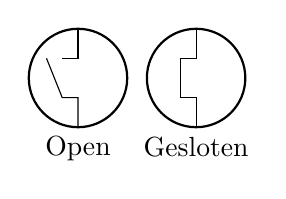
\begin{tikzpicture}
\draw[thick] (0,0) circle(0.625);
\draw (0,-0.625) node[anchor=north]{Open} -- ++(0,0.375) -- ++(-0.2,0) -- ++(-0.2,0.5);
\draw (0,0.625) -- ++(0,-0.375) -- ++(-0.2,0);

\draw[thick] (1.5,0) circle(0.625);
\draw (1.5,-0.625) node[anchor=north]{Gesloten} -- ++(0,0.375) -- ++(-0.2,0) -- ++(0,0.5) -- ++(0.2,0) -- ++(0,0.375);
\end{tikzpicture}
\figlab{switchNotationSwitch}
}
\subfigure[NMOS Schakelaars met stuursignaal] {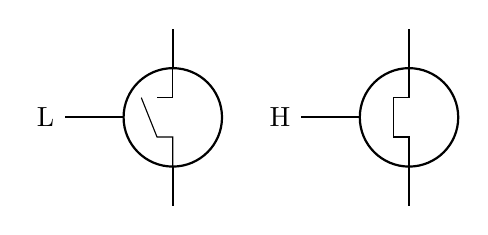
\begin{tikzpicture}
\draw[thick] (0,0) circle(0.625);
\draw (0,-0.625) -- ++(0,0.375) -- ++(-0.2,0) -- ++(-0.2,0.5);
\draw (0,0.625) -- ++(0,-0.375) -- ++(-0.2,0);
\draw[thick] (0,-0.625) -- ++(0,-0.5);
\draw[thick] (0,0.625) -- ++(0,0.5);
\draw[thick] (-0.625,0) -- ++(-0.75,0) node[anchor=east]{L};

\draw[thick] (3,0) circle(0.625);
\draw (3,-0.625) -- ++(0,0.375) -- ++(-0.2,0) -- ++(0,0.5) -- ++(0.2,0) -- ++(0,0.375);
\draw[thick] (3,-0.625) -- ++(0,-0.5);
\draw[thick] (3,0.625) -- ++(0,0.5);
\draw[thick] (2.375,0) -- ++(-0.75,0) node[anchor=east]{H};
\end{tikzpicture}
\figlab{switchNotationControlledNmos}
}
\subfigure[PMOS Schakelaars met stuursignaal] {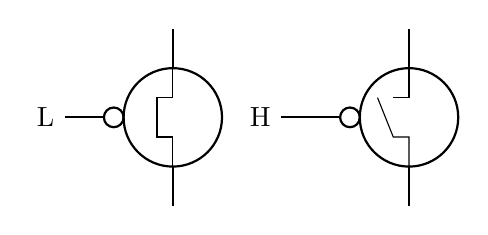
\begin{tikzpicture}
\draw[thick] (6,0) circle(0.625);
\draw[thick] (5.25,0) circle(0.125);
\draw (6,-0.625) -- ++(0,0.375) -- ++(-0.2,0) -- ++(0,0.5) -- ++(0.2,0) -- ++(0,0.375);
\draw[thick] (6,-0.625) -- ++(0,-0.5);
\draw[thick] (6,0.625) -- ++(0,0.5);
\draw[thick] (5.125,0) -- ++(-0.5,0) node[anchor=east]{L};

\draw[thick] (9,0) circle(0.625);
\draw[thick] (8.25,0) circle(0.125);
\draw (9,-0.625) -- ++(0,0.375) -- ++(-0.2,0) -- ++(-0.2,0.5);
\draw (9,0.625) -- ++(0,-0.375) -- ++(-0.2,0);
\draw[thick] (9,-0.625) -- ++(0,-0.5);
\draw[thick] (9,0.625) -- ++(0,0.5);
\draw[thick] (8.125,0) -- ++(-0.75,0) node[anchor=east]{H};
\end{tikzpicture}
\figlab{switchNotationControlledPmos}
}
\caption{Notatie van een schakelaar (met stuursignaal).}
\figlab{switchNotation}
\end{figure}

\subsubsection{Werking van NMOS en PMOS}
\ssslab{nmosPmosWork}
In de vorige subsectie werden twee types automatische schakelaars ge\"introduceerd: NMOS en PMOS. Dit zijn \gtermen{transistoren}{Automatische schakelaars. Een transistor heeft drie verbindingen, de collector en de emittter vormen een schakelaar, en de basis stuurt deze schakelaar aan. Afhankelijk van de soort transistor gelden er andere regels over wanneer de schakelaar gesloten wordt, en volgens welk patroon.} die in bijna elk elektronisch apparaat gebruikt worden. In deze subsectie zullen we de terminologie van een transistor bespreken, en de werking van deze componenten verklaren. Zoals de meeste transistoren hebben een NMOS en PMOS drie aansluitingen: de \gtermen{Source}{Een van de aansluitingen van een transistor. Zoals de naam reeds doet vermoeden wordt de source vaak aan de hoge spanning kant van de voeding aangeschakeld. Afhankelijk van het signaal dat aangelegd wordt op de basis, ontstaat er een verbinding met de drain.}, \gtermen{Gate}{Een van de aansluitingen van een transistor. De gate regelt of er een verbinding tussen de source en de drain tot stand komt.} en \gtermen{Drain}{Een van de aansluitingen van een transistor. De drain wordt meestal aan de lage spannin kant van de voeding aangeschakeld. Afhankelijk van het signaal dat aangelegd wordt op de gate, ontstaat er een verbinding tussen de source en de drain.}, in het Nederlands worden deze aansluitingen ook respectievelijk \stermen{Collector}{Source}, \stermen{Basis}{Gate} en \stermen{Emitter}{Drain} genoemd. Een transistor is eigenlijk niets anders dan een schakelaar tussen de source en drain. De weerstand tussen de source en de drain wordt geregeld volgens de spanning die op de gate staat.

\paragraph{}
\figref{mosWork} toont de concrete werking van NMOS en PMOS transistoren. Voor beide typen transistoren beschouwen we een substraat van siliciumdioxide (SiO$_2$). We kunnen dit substraat zowel positief als negatief \gtermen{doperen}{Het introduceren van alternatieve atomen in een substraat. In de context van een transistor worden substraten van siliciumdioxide negatief of positief edopeerd.}\footnote{Het introduceren van alternatieve atomen.}. Bij NMOS doperen we het substraat hoofdzakelijk positief (p). Bij de ingangen van de source en de drain doperen we negatief (n). Er kan nauwelijks stroom vloeien tussen het negatief en positief gedopeerde substraat. Bijgevolg fungeert de p-laag als een barri\`ere tussen de source en de drain.

\paragraph{}
Indien we echter een positieve spanning aanbrengen op de gate, zullen de negatieve deeltjes in de p-laag zich aangetrokken voelen tot de gate. Er ontstaat een reorganisatie van de p-laag waardoor er een n-laagje gevormd wordt ter hoogte van de gate. Hierdoor ontstaat er een kanaal tussen de source en de drain, waardoor de schakelaar zich sluit. De spanning die tussen de gate en de source moet staan om dit te bereiken wordt de \gtermen{threshold spanning $V_{\mbox{\tiny T}}$}{De spanning die men tussen de gate en de source moet aanleggen bij een NMOS zodat er een verbinding tussen de source en de gate ontstaat.} genoemd. Indien de spanning tussen de gate en de source $V_{\mbox{\tiny GS}}$ dus kleiner is dan $V_{\mbox{\tiny T}}$ is de NMOS schakelaar open, anders is de schakelaar gesloten. Een PMOS transistor werkt op analoge manier, maar dan omgekeerd.

\begin{figure}[hbt]
\centering
\subfigure[NMOS bij $V_{\mbox{\tiny GS}}<V_{\mbox{\tiny T}}$.]{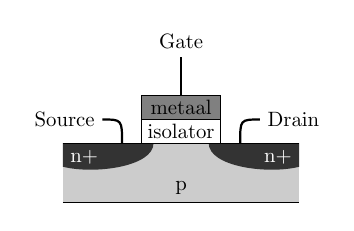
\begin{tikzpicture}
\fill[black!20] (0,0) rectangle (3,0.75);
\fill[black!80] (0,0.75) node[anchor=north west,scale=0.75,white]{n+} -- (0,0.45) .. controls (0.4,0.35) and (1.15,0.45) .. (1.15,0.75) -- cycle;
\fill[black!80] (3,0.75) node[anchor=north east,scale=0.75,white]{n+} -- (3,0.45) .. controls (2.6,0.35) and (1.85,0.45) .. (1.85,0.75) -- cycle;
\draw (1,0.75) rectangle ++(1,0.3);
\draw (1.5,0.9) node[scale=0.75]{isolator};
\filldraw[fill=gray] (1,1.05) rectangle ++(1,0.3);
\draw (1.5,1.2) node[scale=0.75]{metaal};
\draw[thick] (1.5,1.35) -- ++(0,0.5) node[anchor=south,scale=0.75]{Gate};
\draw[thick] (0.75,0.75) .. controls (0.75,1.05) and (0.75,1.05) .. (0.5,1.05) node[anchor=east,scale=0.75]{Source};
\draw[thick] (2.25,0.75) .. controls (2.25,1.05) and (2.25,1.05) .. (2.5,1.05) node[anchor=west,scale=0.75]{Drain};
\draw (0,0) to node[above,midway,scale=0.75]{p} (3,0);
\draw (0,0.75) -- (3,0.75);
\end{tikzpicture}}
\subfigure[NMOS bij $V_{\mbox{\tiny GS}}\geq V_{\mbox{\tiny T}}$.]{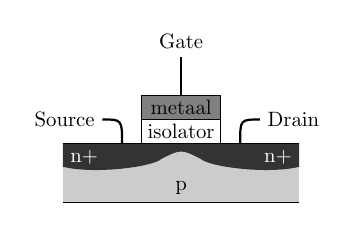
\begin{tikzpicture}
\fill[black!20] (0,0) rectangle (3,0.75);
\fill[black!80] (0,0.75) node[anchor=north west,scale=0.75,white]{n+} -- (0,0.45) .. controls (0.4,0.35) and (1.15,0.45) .. (1.25,0.55)  .. controls (1.5,0.675) and (1.5,0.675) .. (1.75,0.55) .. controls (1.85,0.45) and (2.6,0.35) .. (3,0.45) -- (3,0.75) node[anchor=north east,scale=0.75,white]{n+} -- cycle;
\draw (1,0.75) rectangle ++(1,0.3);
\draw (1.5,0.9) node[scale=0.75]{isolator};
\filldraw[fill=gray] (1,1.05) rectangle ++(1,0.3);
\draw (1.5,1.2) node[scale=0.75]{metaal};
\draw[thick] (1.5,1.35) -- ++(0,0.5) node[anchor=south,scale=0.75]{Gate};
\draw[thick] (0.75,0.75) .. controls (0.75,1.05) and (0.75,1.05) .. (0.5,1.05) node[anchor=east,scale=0.75]{Source};
\draw[thick] (2.25,0.75) .. controls (2.25,1.05) and (2.25,1.05) .. (2.5,1.05) node[anchor=west,scale=0.75]{Drain};
\draw (0,0) to node[above,midway,scale=0.75]{p} (3,0);
\draw (0,0.75) -- (3,0.75);
\end{tikzpicture}}
\subfigure[PMOS bij $V_{\mbox{\tiny GD}}<V_{\mbox{\tiny T}}$.]{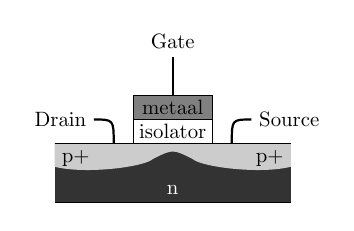
\begin{tikzpicture}
\fill[black!80] (0,0) rectangle (3,0.75);
\fill[black!20] (0,0.75) node[anchor=north west,scale=0.75,black]{p+} -- (0,0.45) .. controls (0.4,0.35) and (1.15,0.45) .. (1.25,0.55)  .. controls (1.5,0.675) and (1.5,0.675) .. (1.75,0.55) .. controls (1.85,0.45) and (2.6,0.35) .. (3,0.45) -- (3,0.75) node[anchor=north east,scale=0.75,black]{p+} -- cycle;
\draw (1,0.75) rectangle ++(1,0.3);
\draw (1.5,0.9) node[scale=0.75]{isolator};
\filldraw[fill=gray] (1,1.05) rectangle ++(1,0.3);
\draw (1.5,1.2) node[scale=0.75]{metaal};
\draw[thick] (1.5,1.35) -- ++(0,0.5) node[anchor=south,scale=0.75]{Gate};
\draw[thick] (0.75,0.75) .. controls (0.75,1.05) and (0.75,1.05) .. (0.5,1.05) node[anchor=east,scale=0.75]{Drain};
\draw[thick] (2.25,0.75) .. controls (2.25,1.05) and (2.25,1.05) .. (2.5,1.05) node[anchor=west,scale=0.75]{Source};
\draw (0,0) to node[above,midway,scale=0.75,white]{n} (3,0);
\draw (0,0.75) -- (3,0.75);
\end{tikzpicture}}
\subfigure[PMOS bij $V_{\mbox{\tiny GD}}\geq V_{\mbox{\tiny T}}$.]{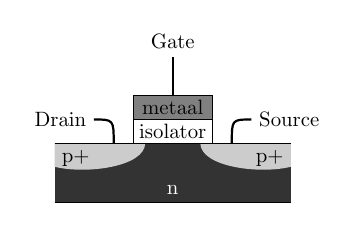
\begin{tikzpicture}
\fill[black!80] (0,0) rectangle (3,0.75);
\fill[black!20] (0,0.75) node[anchor=north west,scale=0.75,black]{p+} -- (0,0.45) .. controls (0.4,0.35) and (1.15,0.45) .. (1.15,0.75) -- cycle;
\fill[black!20] (3,0.75) node[anchor=north east,scale=0.75,black]{p+} -- (3,0.45) .. controls (2.6,0.35) and (1.85,0.45) .. (1.85,0.75) -- cycle;
\draw (1,0.75) rectangle ++(1,0.3);
\draw (1.5,0.9) node[scale=0.75]{isolator};
\filldraw[fill=gray] (1,1.05) rectangle ++(1,0.3);
\draw (1.5,1.2) node[scale=0.75]{metaal};
\draw[thick] (1.5,1.35) -- ++(0,0.5) node[anchor=south,scale=0.75]{Gate};
\draw[thick] (0.75,0.75) .. controls (0.75,1.05) and (0.75,1.05) .. (0.5,1.05) node[anchor=east,scale=0.75]{Drain};
\draw[thick] (2.25,0.75) .. controls (2.25,1.05) and (2.25,1.05) .. (2.5,1.05) node[anchor=west,scale=0.75]{Source};
\draw (0,0) to node[above,midway,scale=0.75,white]{n} (3,0);
\draw (0,0.75) -- (3,0.75);
\end{tikzpicture}}
\caption{Werking van NMOS en PMOS.}
\figlab{mosWork}
\end{figure}

%REVIEW
\subsection{Basispoorten}
Nu we automatische schakelaars kunnen gebruiken,  kunnen we met behulp van NMOS en PMOS de basispoorten implementeren. Eerst zullen we de basispoorten met behulp van NMOS implementeren. Vervolgens zal blijken dat deze implementaties enkele nadelen hebben. Hierdoor zullen we opteren voor implementatie met \termen{CMOS}. CMOS is in feite een combinatie van NMOS en PMOS. We zullen alle schakelingen implementeren in positieve logica. In \secref{negativeLogic} behandelen we nog enkele zaken in verband met negatieve logica.

\subsubsection{Implementatie in NMOS}
\paragraph{NOT}
\figref{notNmos} toont de implementatie van een NOT-poort in NMOS. Als ingang beschouwen we $x$, als uitgang $f$ de $V_{\mbox{\tiny DD}}$ en $V_{\mbox{\tiny SS}}$ zijn lijnen voor de voeding van de poort. Indien we een laag voltage aanbrengen op $x$ is de NMOS transistor open. Hierdoor staat er een hoge spanning op $f$. Indien we echter een hoge spanning op $x$ aanbrengen, zal de transistor zich sluiten. Hierdoor vloeit er stroom tussen $V_{\mbox{\tiny DD}}$ en $V_{\mbox{\tiny SS}}$. Omdat de stroom door $f$ nog andere componenten zal aansturen, zal de stroom bijgevolg verkiezen om door de transistor te stromen, en krijgt $f$ dus een laag potentiaal. Het principe van het verlagen van de spanning door stroom door te laten wordt \termen{Pull-Down Network (PDN)} genoemd. Theoretisch gezien mag dit model mooi lijken, de werkelijkheid verschilt echter. Wanneer de NMOS transistor immers gesloten is, zal er immers nog steeds een kleine weerstand over staan. Deze weerstand noteren we als $R_{\mbox{\tiny on}}$. Dit betekent dat $f$ niet volledig gelijk zal zijn aan $L$. We berekenen de spanning op $f$ dan ook met volgende formule:

\begin{equation}
V_{\mbox{\tiny out}}\left(x=1\right)=\displaystyle\frac{R_{\mbox{\tiny on}}}{R+R_{\mbox{\tiny on}}}V_{\mbox{\tiny DD}}
\end{equation}
Een tweede groot nadeel is dat we bij $x=H$ statisch vermogen verbruiken:
\begin{equation}
P\left(x=1\right)=\displaystyle\frac{V_{\mbox{\tiny DD}}^2}{R+R_{\mbox{\tiny on}}}
\end{equation}

Dit is op energieniveau een grote kost, vooral omdat er in een gemiddelde processor makkelijk miljoenen transistoren zitten. Bovendien zou dit hoge temperaturen genereren. Dit is dan ook de hoofdreden waarom er nauwelijks elektronica ge\"implementeerd wordt met NMOS.

\begin{figure}[hbt]
\centering
\subfigure[x=L, f=H]{\begin{circuitikz}[american resistors]
\node [nmoso] (T) at (0,3) {};
\draw[<-] (0,4.75) node[anchor=west,scale=0.75]{$V_{\mbox{\tiny DD}}\ (H)$} -- (0,4.5);
\draw (0,4.5) to [R,l={\small $R$}] (0,3.5) -- (T.drain);
\draw (0,3.5) -- ++(1,0) node[anchor=west,scale=0.75]{$f=H$};
\draw (T.gate) -- ++(-0.5,0) node[anchor=east,scale=0.75]{$x=L$};
\draw (T.source) -- (0,2.65) node[ground]{};
\draw (0.4,2.3) node[anchor=west,scale=0.75]{$V_{\mbox{\tiny SS}}\ (L)$};
\end{circuitikz}}
\subfigure[x=H, f=L]{\begin{circuitikz}[american resistors]
\node [nmosc] (T) at (0,3) {};
\draw[<-] (0,4.75) node[anchor=west,scale=0.75]{$V_{\mbox{\tiny DD}}\ (H)$} -- (0,4.5);
\draw (0,4.5) to [R,l={\small $R$}] (0,3.5) -- (T.drain);
\draw (0,3.5) -- ++(1,0) node[anchor=west,scale=0.75]{$f=L$};
\draw (T.gate) -- ++(-0.5,0) node[anchor=east,scale=0.75]{$x=H$};
\draw (T.source) -- (0,2.65) node[ground]{};
\draw (0.4,2.3) node[anchor=west,scale=0.75]{$V_{\mbox{\tiny SS}}\ (L)$};
\end{circuitikz}}
\caption{NOT poort ge\"implementeerd in NMOS.}
\figlab{notNmos}
\end{figure}

\paragraph{``Open-drain poort''}
Indien we de weerstand als een extern component beschouwen, en meer NMOS transistoren in parallel aan de draad hangen, kunnen we het gedrag van een AND poort nabootsen, zoals op \figref{openDrainNmos}. Vanaf het moment dat \'e\'en van de transistoren gesloten wordt, lekt de stroom door die transistor, en krijgt $f$ dus een laag niveau. Alle ingangen moeten dus een lage spanning hebben, om een hoge spanning aan de uitgang te verkrijgen. We kunnen dit principe dus zien als een AND waarbij aan alle ingangen een inverter staat. Dit systeem wordt ``\termen{Open-Drain Poort}'' genoemd. En heeft het voordeel dat we een AND kunnen bouwen aan de hand van draden. Deze implementatie is dus goedkoop indien we een AND-poort willen maken met een zeer groot aantal ingangen. Standaard wordt dit soort implementatie dan ook gebruikt in de reset-functionaliteit van elektronica. Meestal wordt er immers een reset procedure aangeroepen indien \'e\'en van de detectoren een fout registreert. In dat geval zal de detector een hoge spanning aan zijn ingang genereren. Dit resulteert een lage uitgang, bij een lage uitgang treed de reset-procedure dan in werking.
\begin{figure}[hbt]
\centering
\begin{circuitikz}[american resistors]
\node [nmosc] (T1) at (-1,2.75) {};
\node [nmosc] (T2) at (-1,0.75) {};
\draw[<-] (0,4.75) node[anchor=west,scale=0.75]{$V_{\mbox{\tiny DD}}\ (H)$} -- (0,4.5);
\draw (0,4.5) to [R,size=0.5,l={\small $R$}] (0,3.5) -- (0,-0.25);
\draw (0,3.5) -| (T1.drain);
\draw (0,1.5) -| (T2.drain);
\draw (0,2.5) -- ++(1,0) node[anchor=west,scale=0.75]{$f$};
\draw (T1.gate) -- ++(-0.25,0) node[anchor=east,scale=0.75]{$x$};
\draw (T1.source) -- ++(0,0) node[ground]{};
\draw (T2.gate) -- ++(-0.25,0) node[anchor=east,scale=0.75]{$y$};
\draw (T2.source) -- ++(0,0) node[ground]{};
\end{circuitikz}
\caption{Open-Drain Poort in NMOS.}
\figlab{openDrainNmos}
\end{figure}
\paragraph{NAND en NOR}
De vorige paragraaf gaf reeds een opzet hoe we een NOR en NAND poort kunnen bouwen. We moeten er eenvoudig weg voor zorgen dat er stroom kan vloeien tussen $V_{\mbox{\tiny DD}}$ en $V_{\mbox{\tiny SS}}$ indien respectievelijk minstens \'e\'en of alle transistoren gesloten worden. \figref{nandNorNmos} toont dan ook de implementaties voor een NAND en NOR poort. Een AND en OR poort kunnen we dan vervolgens synthetiseren door een inverter achter de poort te plaatsen. Deze implementaties maken ook meteen duidelijk waarom een NAND goedkoper is dan een AND.
\begin{figure}
\centering
\subfigure[NAND poort.]{\begin{circuitikz}[american resistors]
\node [nmosc] (T1) at (0,3) {};
\node [nmosc] (T2) at (0,2) {};
\draw[<-] (0,4.75) node[anchor=west,scale=0.75]{$V_{\mbox{\tiny DD}}\ (H)$} -- (0,4.5);
\draw (0,4.5) to [R,l={\small $R$}] (0,3.5) -- (T1.drain);
\draw (0,3.5) -- ++(1,0) node[anchor=west,scale=0.75]{$f$};
\draw (T1.gate) -- ++(-0.5,0) node[anchor=east,scale=0.75]{$x$};
\draw (T1.source) -- (T2.drain);
\draw (T2.gate) -- ++(-0.5,0) node[anchor=east,scale=0.75]{$y$};
\draw (T2.source) -- ++(0,0) node[ground]{};
\end{circuitikz}}
\subfigure[NOR poort.]{\begin{circuitikz}[american resistors]
\node [nmosc] (T1) at (-1,2.5) {};
\node [nmosc] (T2) at (1,2.5) {};
\draw[<-] (0,4.75) node[anchor=west,scale=0.75]{$V_{\mbox{\tiny DD}}\ (H)$} -- (0,4.5);
\draw (0,4.5) to [R,l={\small $R$}] (0,3.5);
\draw (0,3.5) -- ++(1,0) node[anchor=west,scale=0.75]{$f$};
\draw (T1.gate) -- ++(-0.5,0) node[anchor=east,scale=0.75]{$x$};
\draw (T1.drain) |- ++(1,0.25);
\draw (T1.source) |- ++(1,-0.25);
\draw (T2.gate) -- ++(-0.5,0) node[anchor=east,scale=0.75]{$y$};
\draw (T2.drain) |- ++(-1,0.25) -- (0,3.5);
\draw (T2.source) |- ++(-1,-0.25) -- ++(0,-0.25) node[ground]{};
\end{circuitikz}}
\caption{NAND en NOR poort ge\"implementeerd met NMOS.}
\figlab{nandNorNmos}
\end{figure}
\subsubsection{Implementatie in CMOS}
Het grote argument tegen het gebruik van NMOS is dat het veel vermogen nutteloos verbruikt. CMOS biedt hiervoor een oplossing. CMOS is eigenlijk een techniek waarbij we zowel een NMOS als een PMOS transistor gebruiken. Analoog aan het ``Pull-Down Network'' fenomeen van de NMOS, spreken we dan over het ``\termen{Pull-Up Network (PUN)}'' fenomeen bij PMOS.
\paragraph{NOT}Indien we de uitgang $f$ plaatsen tussen een NMOS en PMOS transistor, die we allebei met dezelfde ingang $x$ verbinden, kunnen we een NOT poort implementeren. De uitwerking hiervan staat op \figref{notCmos}. Op het moment dat we een hoge spanning aanleggen op de ingang sluit de NMOS transistor zich, en opent de PMOS transistor zich, hierdoor krijgt de uitgang dezelfde spanning als de ground. Indien we een lage spanning aan de ingang aanleggen is de configuratie van de transistoren omgekeerd, en wordt komt aan de uitgang een spanning $V_{\mbox{\tiny DD}}$ te liggen.
\begin{figure}[hbt]
\centering
\begin{circuitikz}[american resistors]
\node [pmosc] (T1) at (0,3.75) {};
\node [nmoso] (T2) at (0,2.75) {};
\draw[<-] (0,4.5) node[anchor=west,scale=0.75]{$V_{\mbox{\tiny DD}}\ (H)$} -- (0,4);
\draw (0,3.25) -- ++(1,0) node[anchor=west,scale=0.75]{$f=H$};
\draw (T1.source) -- (0,4.5);
\draw (T1.drain) -- (T2.drain);
\draw (T1.gate) -- (T1.gate -| -0.75,0) |- (T2.gate);
\draw (-0.75,3.25) -- ++(-0.5,0) node[anchor=east,scale=0.75]{$x=L$};
\draw (T2.source) -- ++(0,0) node[ground]{};
\begin{scope}[xshift=6 cm]
\node [pmoso] (T1) at (0,3.75) {};
\node [nmosc] (T2) at (0,2.75) {};
\draw[<-] (0,4.5) node[anchor=west,scale=0.75]{$V_{\mbox{\tiny DD}}\ (H)$} -- (0,4);
\draw (0,3.25) -- ++(1,0) node[anchor=west,scale=0.75]{$f=L$};
\draw (T1.source) -- (0,4.5);
\draw (T1.drain) -- (T2.drain);
\draw (T1.gate) -- (T1.gate -| -0.75,0) |- (T2.gate);
\draw (-0.75,3.25) -- ++(-0.5,0) node[anchor=east,scale=0.75]{$x=H$};
\draw (T2.source) -- ++(0,0) node[ground]{};
\end{scope}
\end{circuitikz}
\caption{NOT poort ge\"implementeerd met CMOS.}
\figlab{notCmos}
\end{figure}
\paragraph{NAND en NOR} Ook NAND en NOR poorten hebben hun equivalent in CMOS. \figref{nandNorCmos} toont hun implementatie. Wat opvalt is dat we redelijk eenvoudig het CMOS equivalent kunnen halen uit een NMOS implementatie. Immers is het onderste gedeelte van de NMOS-schakelaars volledig equivalent met de NMOS-implementatie. We plaatsen eenvoudigweg een PMOS circuit boven de uitgang. Dit circuit werkt met duale logica: indien de NMOS verbindingen parallel zijn, zullen we de PMOS transistoren in serie plaatsen, indien de NMOS transistoren in serie stonden, zetten we de PMOS transistoren in parallel. Verder kunnen we de weerstand ook weglaten. Deze weerstand stond er immers alleen om verschillende poorten aan eenzelfde voeding te kunnen hangen. Nu er echter geen stroom vloeit in om het even welke configuratie van de transistoren, is de weerstand dus nagenoeg nutteloos geworden, en brengt deze hoge kosten met zich mee.
\begin{figure}[hbt]
\centering
\subfigure[NAND]{\begin{circuitikz}[american resistors]
\node [pmoso] (T1) at (-1,1) {};
\node [pmoso] (T2) at (1,1) {};
\node [nmosc] (T3) at (0,-0.5) {};
\node [nmosc] (T4) at (0,-1.5) {};
\draw[->] (T1.source) |- ++(1,0.25) -- ++(0,0.5) node[anchor=west,scale=0.75]{$V_{\mbox{\tiny DD}}\ (H)$};
\draw (T2.source) |- ++(-1,0.25);
\draw (T1.drain) |- ++(1,-0.25) -- (0,0);
\draw (T1.gate) -- (T1.gate -| -2,0) node[anchor=east,scale=0.75]{$x$};
\draw (T2.drain) |- ++(-1,-0.25);
\draw (T2.gate) -- ++(-0.5,0) -- (T3.gate -| -0.75,0);
\draw (T4.gate) -- ++(-0.5,0) -- (T1.gate -| -1.75,0);
\draw (T3.gate) -- (T3.gate -| -2,0) node[anchor=east,scale=0.75]{$y$};
\draw (0,0) -- ++(2,0) node[anchor=west,scale=0.75]{$f$};
\draw (0,0) -- (T3.drain);
\draw (T3.source) -- (T4.drain);
\draw (T4.source) -- ++(0,0) node[ground]{};
\end{circuitikz}
\figlab{nandCmos}}
\subfigure[NOR]{\begin{circuitikz}[american resistors]
\node [nmosc] (T1) at (-1,-1) {};
\node [nmosc] (T2) at (1,-1) {};
\node [pmoso] (T3) at (0,0.5) {};
\node [pmoso] (T4) at (0,1.5) {};
%\draw[<-] (0,4.5) node[anchor=west,scale=0.75]{$V_{\mbox{\tiny DD}}\ (H)$} -- (0,4);
\draw[->] (T4.source) -- ++(0,0.25) node[anchor=west,scale=0.75]{$V_{\mbox{\tiny DD}}\ (H)$};
\draw (T2.drain) |- ++(-1,0.25) -- (0,0);
\draw (T1.drain) |- ++(1,0.25);
\draw (T1.source) |- ++(1,-0.25) -- ++(0,-0.25) node[ground]{};
\draw (T2.source) |- ++(-1,-0.25);
\draw (T1.gate) -- (T1.gate -| -2,0) node[anchor=east,scale=0.75]{$y$};
\draw (T2.source) |- ++(-1,-0.25);
\draw (T2.gate) -- ++(-0.5,0) -- (T3.gate -| -0.75,0);
\draw (T4.gate) -- ++(-0.5,0) -- (T1.gate -| -1.75,0);
\draw (T3.gate) -- (T3.gate -| -2,0) node[anchor=east,scale=0.75]{$x$};
\draw (0,0) -- ++(2,0) node[anchor=west,scale=0.75]{$f$};
\draw (0,0) -- (T3.drain);
\draw (T3.source) -- (T4.drain);
\end{circuitikz}
\figlab{norCmos}}
\caption{NAND en NOR poorten ge\"implementeerd met CMOS.}
\figlab{nandNorCmos}
\end{figure}
\paragraph{Uitgangen verbinden}
\label{term:kortsluiting}
Bij NMOS konden we uitgangen met elkaar verbinden, zonder dat dit problemen met zich meebracht, sterker nog, we konden sommige poorten implementeren aan de hand van verbindingen. Een groot nadeel van CMOS is dat dit niet langer mogelijk is. \figref{cmosFail} toont de reden hiervoor. Op het moment dat de ene ingang een hoog potentiaal heeft, en de andere een laag potentiaal ontstaat er immers een kortsluiting. De stroom is in staat om vanaf de $V_{\mbox{\tiny DD}}$ rechtstreeks de aarding te bereiken. Hoewel de transistoren een minimale weerstand hebben, volstaat deze meestal niet. Het gevolg zijn zeer hoge stromen die het elektronische circuit zouden kunnen beschadigen.
\begin{figure}[hbt]
\centering
\begin{circuitikz}[american resistors]
\def\dx{3};
\node [pmosc] (T1) at (0,3.75) {};
\node [nmoso] (T2) at (0,2.75) {};
\draw[<-] (0,4.5) node[anchor=west,scale=0.75]{$V_{\mbox{\tiny DD}}\ (H)$} -- (0,4);
\draw (0,3.25) -| ++(1,-2) -| (\dx+1,3.25);
\draw (T1.source) -- (0,4);
\draw (T1.drain) -- (T2.drain);
\draw (T1.gate) -- (T1.gate -| -0.75,0) |- (T2.gate);
\draw (-0.75,3.25) -- ++(-0.5,0);
\draw (T2.source) -- ++(0,0) node[ground]{};
\node [pmoso] (T3) at (\dx,3.75) {};
\node [nmosc] (T4) at (\dx,2.75) {};
\draw[<-] (\dx,4.5) node[anchor=west,scale=0.75]{$V_{\mbox{\tiny DD}}\ (H)$} -- (\dx,4);
\draw (\dx,3.25) -- ++(1,0);
\draw (T3.source) -- (\dx,4);
\draw (T3.drain) -- (T4.drain);
\draw (T3.gate) -- (T3.gate -| \dx-0.75,0) |- (T4.gate);
\draw (\dx-0.75,3.25) -- ++(-0.5,0);
\draw (T4.source) -- ++(0,0) node[ground]{};
\draw[dotted,thick,rounded corners,->] (0.35,4.1) -- (0.35,3.6) -| (1.35,1.6) -| (\dx+0.65,2.9) -| (\dx+0.35,2);
\end{circuitikz}
\caption{Kortsluiting bij wired poort implementaties met CMOS.}
\figlab{cmosFail}
\end{figure}
\subsection{Complexe poorten}
\begin{figure}[hbt]
\centering
\subfigure[AOI op poortniveau.]{\begin{tikzpicture}[circuit logic US]
\node[and gate,rotate=90] (A1) at (-0.85,0) {};
\draw (A1.input 1) -- (A1.input 1 |- 0,-1.75) node[anchor=north]{$a$};
\draw (A1.input 2) -- (A1.input 2 |- 0,-2.25) node[anchor=north]{$b$};
\node[and gate,inputs={normal,normal,normal},rotate=90] (A2) at (0.85,0) {};
\draw (A2.input 1) -- (A2.input 1 |- 0,-1.75) node[anchor=north]{$x$};
\draw (A2.input 2) -- (A2.input 2 |- 0,-2) node[anchor=north]{$y$};
\draw (A2.input 3) -- (A2.input 3 |- 0,-2.25) node[anchor=north]{$z$};
\node[nor gate,rotate=90] (NO) at (0,3) {};
\draw (NO.output) -- ++(0,1.5) node[anchor=south]{$f$};
\draw (A1.output) -- ++(0,1.4) -| (NO.input 1);
\draw (A2.output) -- ++(0,1.4) -| (NO.input 2);
\end{tikzpicture}
\figlab{aoiExample}}
\subfigure[AOI op CMOS-niveau.]{
\begin{circuitikz}
\def\dxy{1.5};
\def\dg{0.2};
\def\ds{0.1};
\node[pmoso] (PB1) at (-0.5*\dxy,2*\dxy) {};
\draw (PB1.gate) -- ++(-\dg,0) node[anchor=east,scale=0.75]{$a$};
\node[pmoso] (PB2) at (0.5*\dxy,2*\dxy) {};
\draw (PB2.gate) -- ++(-\dg,0) node[anchor=east,scale=0.75]{$b$};

\coordinate (SPBb) at (0,2.5*\dxy-\ds);
\draw (PB1.source) |- (SPBb);
\draw (PB2.source) |- (SPBb);
\draw[->] (SPBb) -- ++(0,0.5) node[anchor=west,scale=0.75]{$V_{\mbox{\tiny DD}}\ (H)$};
\coordinate (SPBe) at (0,1.5*\dxy+\ds);
\draw (PB1.drain) |- (SPBe);
\draw (PB2.drain) |- (SPBe);

\node[pmoso] (PA1) at (-\dxy,1*\dxy) {};
\draw (PA1.gate) -- ++(-\dg,0) node[anchor=east,scale=0.75]{$x$};
\node[pmoso] (PA2) at (0,1*\dxy) {};
\draw (PA2.gate) -- ++(-\dg,0) node[anchor=east,scale=0.75]{$y$};
\node[pmoso] (PA3) at (\dxy,1*\dxy) {};
\draw (PA3.gate) -- ++(-\dg,0) node[anchor=east,scale=0.75]{$z$};

\coordinate (SPAb) at (0,1.5*\dxy-\ds);
\draw (PA1.source) |- (SPAb);
\draw (PA2.source) |- (SPAb);
\draw (PA3.source) |- (SPAb);
\draw (SPBe) -- (SPAb);

\coordinate (SPAe) at (0,0.5*\dxy+\ds);
\draw (PA1.drain) |- (SPAe);
\draw (PA2.drain) |- (SPAe);
\draw (PA3.drain) |- (SPAe);

\fill (SPAe) circle (0.05 cm);
\fill (SPAb) circle (0.05 cm);

\draw (0,0.25) -- ++(2,0) node[anchor=west,scale=0.75]{$f$};

\node[nmosc] (NA1) at (0.5*\dxy,-0.5*\dxy) {};
\draw (NA1.gate) -- ++(-\dg,0) node[anchor=east,scale=0.75]{$x$};
\node[nmosc] (NA2) at (0.5*\dxy,-1.5*\dxy) {};
\draw (NA2.gate) -- ++(-\dg,0) node[anchor=east,scale=0.75]{$y$};
\node[nmosc] (NA3) at (0.5*\dxy,-2.5*\dxy) {};
\draw (NA3.gate) -- ++(-\dg,0) node[anchor=east,scale=0.75]{$z$};
\node[nmosc] (NB1) at (-0.5*\dxy,-\dxy) {};
\draw (NB1.gate) -- ++(-\dg,0) node[anchor=east,scale=0.75]{$a$};
\node[nmosc] (NB2) at (-0.5*\dxy,-2*\dxy) {};
\draw (NB2.gate) -- ++(-\dg,0) node[anchor=east,scale=0.75]{$b$};

\coordinate (SNAb) at (0,-\ds);

\draw (SPAe) -- (SNAb);

\draw (SNAb) -| (NA1.drain);
\draw (SNAb) -| (NB1.drain);
\draw (NA1.source) -- (NA2.drain);
\draw (NA2.source) -- (NA3.drain);
\draw (NB1.source) -- (NB2.drain);

\coordinate (SNAe) at (0,-3*\dxy+\ds);

\draw (NB2.source) |- (SNAe);
\draw (NA3.source) |- (SNAe);
\draw (SNAe) node[ground]{};
\end{circuitikz}
\figlab{aoiCmos}
}
\subfigure[OAI op poortniveau.]{\begin{tikzpicture}[circuit logic US]
\node[or gate,rotate=90] (A1) at (-0.85,0) {};
\draw (A1.input 1) -- (A1.input 1 |- 0,-1.75) node[anchor=north]{$a$};
\draw (A1.input 2) -- (A1.input 2 |- 0,-2.25) node[anchor=north]{$b$};
\node[or gate,inputs={normal,normal,normal},rotate=90] (A2) at (0.85,0) {};
\draw (A2.input 1) -- (A2.input 1 |- 0,-1.75) node[anchor=north]{$x$};
\draw (A2.input 2) -- (A2.input 2 |- 0,-2) node[anchor=north]{$y$};
\draw (A2.input 3) -- (A2.input 3 |- 0,-2.25) node[anchor=north]{$z$};
\node[nand gate,rotate=90] (NO) at (0,3) {};
\draw (NO.output) -- ++(0,1.5) node[anchor=south]{$f$};
\draw (A1.output) -- ++(0,1.4) -| (NO.input 1);
\draw (A2.output) -- ++(0,1.4) -| (NO.input 2);
\end{tikzpicture}
\figlab{oaiExample}}
\subfigure[OAI op CMOS-niveau.]{
\begin{circuitikz}
\def\dxy{1.5};
\def\dg{0.2};
\def\ds{0.1};
\node[nmosc] (PB1) at (-0.5*\dxy,-2*\dxy) {};
\draw (PB1.gate) -- ++(-\dg,0) node[anchor=east,scale=0.75]{$a$};
\node[nmosc] (PB2) at (0.5*\dxy,-2*\dxy) {};
\draw (PB2.gate) -- ++(-\dg,0) node[anchor=east,scale=0.75]{$b$};

\coordinate (SPBb) at (0,-2.5*\dxy+\ds);
\draw (PB1.source) |- (SPBb);
\draw (PB2.source) |- (SPBb);
\draw (SPBb) node[ground] {};
\coordinate (SPBe) at (0,-1.5*\dxy-\ds);
\draw (PB1.drain) |- (SPBe);
\draw (PB2.drain) |- (SPBe);

\node[nmosc] (PA1) at (-\dxy,-1*\dxy) {};
\draw (PA1.gate) -- ++(-\dg,0) node[anchor=east,scale=0.75]{$x$};
\node[nmosc] (PA2) at (0,-1*\dxy) {};
\draw (PA2.gate) -- ++(-\dg,0) node[anchor=east,scale=0.75]{$y$};
\node[nmosc] (PA3) at (\dxy,-1*\dxy) {};
\draw (PA3.gate) -- ++(-\dg,0) node[anchor=east,scale=0.75]{$z$};

\coordinate (SPAb) at (0,-1.5*\dxy+\ds);
\draw (PA1.source) |- (SPAb);
\draw (PA2.source) |- (SPAb);
\draw (PA3.source) |- (SPAb);
\draw (SPBe) -- (SPAb);

\coordinate (SPAe) at (0,-0.5*\dxy-\ds);
\draw (PA1.drain) |- (SPAe);
\draw (PA2.drain) |- (SPAe);
\draw (PA3.drain) |- (SPAe);

\fill (SPAe) circle (0.05 cm);
\fill (SPAb) circle (0.05 cm);

\draw (0,-0.25) -- ++(2,0) node[anchor=west,scale=0.75]{$f$};

\node[pmoso] (NA1) at (0.5*\dxy,0.5*\dxy) {};
\draw (NA1.gate) -- ++(-\dg,0) node[anchor=east,scale=0.75]{$x$};
\node[pmoso] (NA2) at (0.5*\dxy,1.5*\dxy) {};
\draw (NA2.gate) -- ++(-\dg,0) node[anchor=east,scale=0.75]{$y$};
\node[pmoso] (NA3) at (0.5*\dxy,2.5*\dxy) {};
\draw (NA3.gate) -- ++(-\dg,0) node[anchor=east,scale=0.75]{$z$};
\node[pmoso] (NB1) at (-0.5*\dxy,\dxy) {};
\draw (NB1.gate) -- ++(-\dg,0) node[anchor=east,scale=0.75]{$a$};
\node[pmoso] (NB2) at (-0.5*\dxy,2*\dxy) {};
\draw (NB2.gate) -- ++(-\dg,0) node[anchor=east,scale=0.75]{$b$};

\coordinate (SNAb) at (0,\ds);

\draw (SPAe) -- (SNAb);

\draw (SNAb) -| (NA1.drain);
\draw (SNAb) -| (NB1.drain);
\draw (NA1.source) -- (NA2.drain);
\draw (NA2.source) -- (NA3.drain);
\draw (NB1.source) -- (NB2.drain);

\coordinate (SNAe) at (0,3*\dxy-\ds);

\draw (NB2.source) |- (SNAe);
\draw (NA3.source) |- (SNAe);
\draw[->] (SNAe) -- ++(0,0.5) node[anchor=west,scale=0.75]{$V_{\mbox{\tiny DD}}\ (H)$};
\end{circuitikz}
\figlab{oaiCmos}
}
\caption{AND-OR-Inverter (AOI) en OR-AND-Inverter (OAI) in CMOS.}
\figlab{aoiOai}
\end{figure}
In hoofdstuk \ref{ch:basis} hadden we het reeds over de XOR-poort. Een poort die 1 teruggeeft als de twee ingangen niet gelijk zijn aan elkaar. Deze poort hadden we toen ge\"implementeerd met een ingewikkeld schema van poorten. Omdat we echter op transistor niveau werken, kunnen we verschillende complexe poorten toch relatief simpel implementeren. In de volgende subsecties zullen we eerst de \termen{AND-OR-Invert (AOI)} en \termen{OR-AND-Invert (OAI)} implementeren. Deze schakelingen worden relatief vaak gebruikt, om bijvoorbeeld XOR en \termen{XNOR} poorten te implementeren.
\subsubsection{AND-OR-Invert (AOI)}
Een veelgebruikt component is een AND-OR-Inverter. Dit is een component die we op poort-niveau kunnen beschrijven als een tweelagige structuur waarbij de ingangen eerst door een reeks AND-poorten gaan. De uitgangen van de AND-poorten vormen op hun beurt de ingangen van een NOR-poort. Een concreet voorbeeld hiervan staat op \figref{aoiExample}. Indien we echter de schakeling zouden bouwen zoals we dit voorstellen op poortniveau\footnote{We substitueren dus iedere poort door zijn equivalent in CMOS.}, hebben we 18 transistoren nodig. Een effici\"entere manier is het implementeren van een nieuw component de AOI zoals op \figref{aoiCmos}. Hierbij hebben we slechts 10 transistoren nodig. Bovendien hebben we de implementatie gereduceerd tot \'e\'en laag. Hierdoor wordt de vertraging van de component ook teruggedrongen.
\subsubsection{OR-AND-Invert (OAI)}
De tegenhanger van de AND-OR-Inverter is de OR-AND-Inverter. \figref{oaiExample} toont een voorbeeld van dit type component. Naar analogie met de AOI bestaat deze component op poortniveau opnieuw uit twee lagen, ditmaal gaan de ingangen door een reeks OR poorten waarbij hun uitgangen dan weer de invoer van een NAND poort vormen. Opnieuw kunnen we door een implementatie in CMOS het aantal transistoren van 18 naar 10 reduceren.
\subsubsection{Andere veelgebruikte poorten}
Naast de NOT, NAND, NOR, AOI en OAI poorten, worden er nog enkele andere poorten frequent gebruikt. De implementatie van deze poorten wordt weergegeven in \figref{alternativeGatesCmos}. In de volgende paragrafen wordt hun nut en werking kort toegelicht.
\begin{figure}[hbt]
\centering
\subfigure[Buffer]{\begin{tikzpicture}[circuit logic US]
\node [buffer gate,scale=0.75] (B) at (-1,0) {};
\node [not gate,scale=0.75] (N1) at (1,0) {};
\node [not gate,scale=0.75] (N2) at (2,0) {};
\draw (N2.output) -- ++(0.25,0);
\draw (N1.output) -- (N2.input);
\draw (N1.input) -- ++(-0.25,0);
\draw (B.output) -- ++(0.25,0);
\draw (B.input) -- ++(-0.25,0);
\draw (0,0) node{$\equiv$};
\begin{scope}[xshift=1 cm, yshift=-3 cm,xscale=0.75]
\coordinate (F0) at (-3,0);
\coordinate (I) at (-2,0);
\draw (F0) node[anchor=east,scale=0.75]{$x$} -- (I);
\node [pmoso] (P1) at (-1,0.75) {};
\draw (I) |- (P1.gate);
\draw[->] (P1.source) -- ++(0,0.5) node[anchor=west,scale=0.75]{$V_{\mbox{\tiny DD}}$};
\node [nmosc] (N1) at (-1,-0.75) {};
\draw (I) |- (N1.gate);
\draw (N1.source) node [ground] {};
\draw (N1.drain) -- (P1.drain);
\node [pmosc] (P2) at (1,0.75) {};
\coordinate (F1) at (-1,0);
\coordinate (O) at (0,0);
\draw (F1) -- (O);
\draw[->] (P2.source) -- ++(0,0.5) node[anchor=west,scale=0.75]{$V_{\mbox{\tiny DD}}$};
\draw (O) |- (P2.gate);
\node [nmoso] (N2) at (1,-0.75) {};
\draw (O) |- (N2.gate);
\draw (N2.source) node [ground] {};
\draw (N2.drain) -- (P2.drain);
\coordinate (F2) at (1,0);
\draw (F2) -- ++(1,0) node[anchor=west,scale=0.75]{$f$};
\end{scope}
\end{tikzpicture}
\figlab{bufferCmos}
}
\subfigure[AND-poort]{\begin{tikzpicture}[circuit logic US]
\node [and gate,scale=0.75] (B) at (-1,0) {};
\node [nand gate,scale=0.75] (N1) at (1,0) {};
\node [not gate,scale=0.75] (N2) at (2,0) {};
\draw (N2.output) -- ++(0.25,0);
\draw (N1.output) -- (N2.input);
\draw (N1.input 1) -- ++(-0.25,0);
\draw (N1.input 2) -- ++(-0.25,0);
\draw (B.output) -- ++(0.25,0);
\draw (B.input 1) -- ++(-0.25,0);
\draw (B.input 2) -- ++(-0.25,0);
\draw (0,0) node{$\equiv$};
\begin{scope}[xshift=0.25 cm, yshift=-3 cm,xscale=0.75]
\node [pmoso] (P1) at (-1,0.75) {};
\draw (P1.gate) -- ++(-0.5,0) node[anchor=east,scale=0.75]{$x$};
\node [pmoso] (P1b) at (-1,1.75) {};
\draw (P1b.gate) -- ++(-0.5,0) node[anchor=east,scale=0.75]{$y$};
\draw (P1b.drain) -- (P1.source);
\draw[->] (P1b.source) -- ++(0,0.5) node[anchor=west,scale=0.75]{$V_{\mbox{\tiny DD}}$};
\node [nmosc] (N1) at (-2,-0.65) {};
\draw (N1.gate) -- ++(-0.5,0) node[anchor=east,scale=0.75]{$x$};
\draw (N1.source) |- ++(1,-0.1) node [ground] {};
\coordinate (O) at (1,0);
\coordinate (Fb) at (-1,-0.2);
\coordinate (F1) at (-1,0);
\draw (P1.drain) -- (F1) -- (Fb) -| (N1.drain);
\node [nmosc] (N1b) at (0,-0.65) {};
\draw (N1b.gate) -- ++(-0.5,0) node[anchor=east,scale=0.75]{$y$};
\draw (Fb) -| (N1b.drain);
\draw (N1b.source) |- ++(-1,-0.1);
\node [pmosc] (P2) at (2,0.75) {};
\draw (F1) -- (O);
\draw[->] (P2.source) -- ++(0,0.5) node[anchor=west,scale=0.75]{$V_{\mbox{\tiny DD}}$};
\draw (O) |- (P2.gate);
\node [nmoso] (N2) at (2,-0.75) {};
\draw (O) |- (N2.gate);
\draw (N2.source) node [ground] {};
\draw (N2.drain) -- (P2.drain);
\coordinate (F2) at (2,0);
\draw (F2) -- ++(1,0) node[anchor=west,scale=0.75]{$f$};
\end{scope}
\end{tikzpicture}
\figlab{andCmos}
}
\subfigure[OR-poort]{\begin{tikzpicture}[circuit logic US]
\node [or gate,scale=0.75] (B) at (-1,0) {};
\node [nor gate,scale=0.75] (N1) at (1,0) {};
\node [not gate,scale=0.75] (N2) at (2,0) {};
\draw (N2.output) -- ++(0.25,0);
\draw (N1.output) -- (N2.input);
\draw (N1.input 1) -- ++(-0.25,0);
\draw (N1.input 2) -- ++(-0.25,0);
\draw (B.output) -- ++(0.25,0);
\draw (B.input 1) -- ++(-0.25,0);
\draw (B.input 2) -- ++(-0.25,0);
\draw (0,0) node{$\equiv$};
\begin{scope}[xshift=0.25 cm, yshift=-3 cm,xscale=0.75]
\node [pmoso] (P1) at (-2,1.65) {};
\draw (P1.gate) -- ++(-0.5,0) node[anchor=east,scale=0.75]{$x$};
\node [pmoso] (P1b) at (0,1.65) {};
\draw (P1b.gate) -- ++(-0.4,0) node[anchor=east,scale=0.75]{$y$};
\draw (P1.source) |- ++(1,0.1);
\draw[->] (P1b.source) |- ++(-1,0.1) -- ++(0,0.5) node[anchor=west,scale=0.75]{$V_{\mbox{\tiny DD}}$};
\node [nmosc] (N1) at (-1,0.25) {};
\draw (N1.gate) -- ++(-0.5,0) node[anchor=east,scale=0.75]{$x$};
\coordinate (O) at (1,0);
\coordinate (Fb) at (-1,1.2);
\draw (P1b.drain) |- (Fb);
\coordinate (F1) at (-1,1);
\draw (P1.drain) |- (Fb) -- (F1) -- (N1.drain);
\node [nmosc] (N1b) at (-1,-0.75) {};
\draw (N1.source) -- (N1b.drain);
\draw (N1b.source) node [ground] {};
\draw (N1b.gate) -- ++(-0.5,0) node[anchor=east,scale=0.75]{$y$};
\node [pmosc] (P2) at (2,0.75) {};
\draw (F1) -- ++(1,0) |- (O);
\draw[->] (P2.source) -- ++(0,0.5) node[anchor=west,scale=0.75]{$V_{\mbox{\tiny DD}}$};
\draw (O) |- (P2.gate);
\node [nmoso] (N2) at (2,-0.75) {};
\draw (O) |- (N2.gate);
\draw (N2.source) node [ground] {};
\draw (N2.drain) -- (P2.drain);
\coordinate (F2) at (2,0);
\draw (F2) -- ++(1,0) node[anchor=west,scale=0.75]{$f$};
\end{scope}
\end{tikzpicture}
\figlab{orCmos}
}
\subfigure[XOR-poort]{\begin{tikzpicture}[circuit logic US]
\node [xor gate,scale=0.75] (X) at (-1,0) {};
\draw (X.output) -- ++(0.25,0);
\draw (X.input 1) -- ++(-0.25,0);
\draw (X.input 2) -- ++(-0.25,0);
\draw (0,0) node{$\equiv$};
\node [nand gate,scale=0.75] (NA) at (3,0) {};
\draw (NA.output) -- ++(0.5,0);
\node [or gate,scale=0.75] (O1) at (2,0.5) {};
\node [or gate,scale=0.75] (O2) at (2,-0.5) {};
\draw (O1.output) -- ++(0.1,0) |- (NA.input 1);
\draw (O2.output) -- ++(0.1,0) |- (NA.input 2);
\node [not gate,scale=0.35] (N1) at (O1.input 1 -| 1,0) {};
\node [not gate,scale=0.35] (N2) at (O2.input 1 -| 1,0) {};
\draw (N1.output) -- (O1.input 1);
\draw (N2.output) -- (O2.input 1);
\draw (N1.input) -- ++(-0.5,0);
\draw (N2.input) -- ++(-0.5,0);
\draw (N2.input -| 0.8,0) |- (O1.input 2);
\draw (N1.input -| 0.65,0) |- (O2.input 2);
\begin{scope}[xshift=0.25 cm, yshift=-5.5 cm,xscale=0.75,yscale=0.8]
\def\dxs{4};
\foreach\l/\lt/\x in {A/x/0,B/y/\dxs} {
  \coordinate (F0\l) at (-3,\x+0.1);
  \coordinate (I) at (-2,\x+0.1);
  \fill (I) circle (0.06 cm);
  \coordinate (O\l0) at (1,\x+0.1);
  \draw (F0\l) node[anchor=east,scale=0.75]{$\lt$} -- (I) -- (O\l0);
  \node [pmoso] (P1\l) at (-1,0.75+\x) {};
  \draw (I) |- (P1\l.gate);
  \draw[->] (P1\l.source) -- ++(0,0.5) node[anchor=west,scale=0.75]{$V_{\mbox{\tiny DD}}$};
  \node [nmosc] (N1\l) at (-1,\x-0.75) {};
  \draw (I) |- (N1\l.gate);
  \draw (N1\l.source) node [ground] {};
  \draw (N1\l.drain) -- (P1\l.drain);
  \coordinate (F1\l) at (-1,\x-0.1);
  \coordinate (O\l1) at (0,\x-0.1);
  \draw (F1\l) -- (O\l1);
}
\begin{scope}[xshift=3 cm]
\node[pmoso] (PaAA) at (-1,\dxs+0.65) {};
\node[pmoso] (PaBA) at (1,\dxs+0.65) {};
\node[pmosc] (PaAB) at (-1,\dxs-0.95) {};
\node[pmosc] (PaBB) at (1,\dxs-0.95) {};
\draw[->] (PaAA.source) |- ++(1,0.1) -- ++(0,0.5) node[anchor=west,scale=0.75]{$V_{\mbox{\tiny DD}}$};
\draw (PaBA.source) |- ++(-1,0.1);
\draw (PaAA.drain) -- (PaAB.source);
\draw (PaBA.drain) -- (PaBB.source);

\coordinate (Mid) at (0,0.5*\dxs);
\coordinate (MidT) at (0,0.5*\dxs+0.4);
\draw (PaAB.drain) |- (MidT);
\draw (PaBB.drain) |- (MidT);
\coordinate (MidB) at (0,0.5*\dxs-0.4);
\draw (MidB) -- (MidT);
\draw (Mid) -- ++(2,0) node[anchor=west,scale=0.75]{$f$};

\node[nmosc] (NaAA) at (-1,0.95) {};
\node[nmoso] (NaBA) at (1,0.95) {};
\draw (NaAA.drain) |- (MidB);
\draw (NaBA.drain) |- (MidB);
\node[nmoso] (NaAB) at (-1,-0.65) {};
\node[nmosc] (NaBB) at (1,-0.65) {};
\draw (NaAB.source) |- ++(1,-0.1) node[ground]{};
\draw (NaBB.source) |- ++(-1,-0.1);
\coordinate (Nmt) at (0,0.25);
\coordinate (Nmb) at (0,0.05);
\draw (Nmt) -- (Nmb);
\draw (Nmb) -| (NaAB.drain);
\draw (Nmb) -| (NaBB.drain);
\draw (Nmt) -| (NaAA.source);
\draw (Nmt) -| (NaBA.source);
\draw (OB0) |- (PaAA.gate);
\draw (OB1) -- ++(2.75,0) |- (PaBB.gate);
\coordinate (yn) at (-2.25,0 |- OB0);
\coordinate (yi) at (-0.25,0 |- PaBB.gate);
\coordinate (xn) at (OA0 |- NaAA.gate);
\coordinate (xnc) at (xn -| -1.85,0);
\draw (xnc) |- ++(1.5,3.1) |- (PaBA.gate);
\draw (OA0) |- (NaAA.gate);
\draw (OA1) |- (NaAB.gate);
\draw (OA1) |- (PaAB.gate);
\draw (yi) |- (NaBA.gate);
\draw (yn) |- (0.25,-1.5) |- (NaBB.gate);
\end{scope}
\end{scope}
\end{tikzpicture}
\figlab{xorCmos}
}
\subfigure[XNOR-poort]{\begin{tikzpicture}[circuit logic US]
\node [xnor gate,scale=0.75] (X) at (-1,0) {};
\draw (X.output) -- ++(0.25,0);
\draw (X.input 1) -- ++(-0.25,0);
\draw (X.input 2) -- ++(-0.25,0);
\draw (0,0) node{$\equiv$};
\node [nor gate,scale=0.75] (NA) at (3,0) {};
\draw (NA.output) -- ++(0.5,0);
\node [and gate,scale=0.75] (O1) at (2,0.5) {};
\node [and gate,scale=0.75] (O2) at (2,-0.5) {};
\draw (O1.output) -- ++(0.1,0) |- (NA.input 1);
\draw (O2.output) -- ++(0.1,0) |- (NA.input 2);
\node [not gate,scale=0.35] (N1) at (O1.input 1 -| 1,0) {};
\node [not gate,scale=0.35] (N2) at (O2.input 1 -| 1,0) {};
\draw (N1.output) -- (O1.input 1);
\draw (N2.output) -- (O2.input 1);
\draw (N1.input) -- ++(-0.5,0);
\draw (N2.input) -- ++(-0.5,0);
\draw (N2.input -| 0.8,0) |- (O1.input 2);
\draw (N1.input -| 0.65,0) |- (O2.input 2);

\begin{scope}[xshift=0.25 cm, yshift=-5.5 cm,xscale=0.75,yscale=0.8]
\def\dxs{4};
\foreach\l/\lt/\x in {A/x/0,B/y/\dxs} {
  \coordinate (F0\l) at (-3,\x+0.1);
  \coordinate (I) at (-2,\x+0.1);
  \fill (I) circle (0.06 cm);
  \coordinate (O\l0) at (1,\x+0.1);
  \draw (F0\l) node[anchor=east,scale=0.75]{$\lt$} -- (I) -- (O\l0);
  \node [pmoso] (P1\l) at (-1,0.75+\x) {};
  \draw (I) |- (P1\l.gate);
  \draw[->] (P1\l.source) -- ++(0,0.5) node[anchor=west,scale=0.75]{$V_{\mbox{\tiny DD}}$};
  \node [nmosc] (N1\l) at (-1,\x-0.75) {};
  \draw (I) |- (N1\l.gate);
  \draw (N1\l.source) node [ground] {};
  \draw (N1\l.drain) -- (P1\l.drain);
  \coordinate (F1\l) at (-1,\x-0.1);
  \coordinate (O\l1) at (0,\x-0.1);
  \draw (F1\l) -- (O\l1);
}
\begin{scope}[xshift=3 cm]
\node[pmoso] (PaAA) at (-1,\dxs+0.65) {};
\node[pmosc] (PaBA) at (1,\dxs+0.65) {};
\node[pmosc] (PaAB) at (-1,\dxs-0.95) {};
\node[pmoso] (PaBB) at (1,\dxs-0.95) {};
\draw[->] (PaAA.source) |- ++(1,0.1) -- ++(0,0.5) node[anchor=west,scale=0.75]{$V_{\mbox{\tiny DD}}$};
\draw (PaBA.source) |- ++(-1,0.1);

\coordinate (Pmt) at (0,\dxs-0.25);
\coordinate (Pmb) at (0,\dxs-0.05);
\draw (Pmt) -- (Pmb);
\draw (Pmb) -| (PaAA.drain);
\draw (Pmb) -| (PaBA.drain);
\draw (Pmt) -| (PaAB.source);
\draw (Pmt) -| (PaBB.source);

\coordinate (Mid) at (0,0.5*\dxs);
\coordinate (MidT) at (0,0.5*\dxs+0.4);
\draw (PaAB.drain) |- (MidT);
\draw (PaBB.drain) |- (MidT);
\coordinate (MidB) at (0,0.5*\dxs-0.4);
\draw (MidB) -- (MidT);
\draw (Mid) -- ++(2,0) node[anchor=west,scale=0.75]{$f$};

\node[nmosc] (NaAA) at (-1,0.95) {};
\node[nmoso] (NaBA) at (1,0.95) {};
\draw (NaAA.drain) |- (MidB);
\draw (NaBA.drain) |- (MidB);
\node[nmoso] (NaAB) at (-1,-0.65) {};
\node[nmosc] (NaBB) at (1,-0.65) {};
\draw (NaAA.source) -- (NaAB.drain);
\draw (NaBA.source) -- (NaBB.drain);

\draw (NaAB.source) |- ++(1,-0.1) node[ground]{};
\draw (NaBB.source) |- ++(-1,-0.1);

\coordinate (MidOB1) at (OB1 -| -2.5,0);
\draw (OB1) -- (MidOB1);
\draw (PaAB.gate -| MidOB1) |- (PaAB.gate);
\draw (MidOB1) |- (Mid -| -0.25,0) |- (NaBA.gate);
\draw (OB0) |- (PaAA.gate);
\draw (OB0) |- (NaAA.gate);
\draw (OA1) |- (NaAB.gate);
\draw (OA0) -- (0.25,0 |- OA0) |- (PaBB.gate);
\draw (0.25,0 |- OA0) |- (NaBB.gate);
\draw (OA1) |- (0.25,\dxs+1.5) |- (PaBA.gate);

%\draw (OB0) |- (PaAA.gate);
%\draw (OB1) -- ++(2.75,0) |- (PaBB.gate);
%\coordinate (yn) at (-2.25,0 |- OB0);
%\coordinate (yi) at (-0.25,0 |- PaBB.gate);
%\coordinate (xn) at (OA0 |- NaAA.gate);
%\coordinate (xnc) at (xn -| -1.85,0);
%\draw (xnc) |- ++(1.5,3.1) |- (PaBA.gate);
%\draw (OA0) |- (NaAA.gate);
%\draw (OA1) |- (NaAB.gate);
%\draw (OA1) |- (PaAB.gate);
%\draw (yi) |- (NaBA.gate);
%\draw (yn) |- (0.25,-1.5) |- (NaBB.gate);
\end{scope}
\end{scope}

\end{tikzpicture}
\figlab{xnorCmos}
}
\caption{Implementatie van populaire alternatieve poorten in CMOS.}
\figlab{alternativeGatesCmos}
\end{figure}
\paragraph{Buffer}
Een \termen{buffer} of \termen{driver} is een speciaal type poort met \'e\'en ingang waarbij de uitgang dezelfde waarde heeft als de ingang. Men zou dus in principe een buffer kunnen vervangen door een draad. Toch wordt een buffer frequent gebruikt, indien een bepaalde draad verbonden wordt met vele ingangen van andere poorten. In dat geval immers, zou de spanning op deze draad verlaagd worden. Een buffer dient dus om bij complexe circuits een signaal over een groot aantal componenten te kunnen verspreiden, waar een eenvoudige vertakking zou falen. \figref{bufferCmos} toont de notatie en de implementatie van een buffer. We implementeren een buffer meestal met twee opeenvolgende inverters.
\paragraph{AND-poort}
We hebben een AND-poort reeds voldoende ge\"introduceerd om te weten wat deze component doet. Als we naar \figref{andCmos} kijken, zien we dat we deze poort implementeren door een NOT-poort aan de uitgang van een NAND-poort te plaatsen. Dit verklaart ook meteen waarom we de voorkeur zullen geven aan inverterende poorten: een NAND werkt sneller en is bovendien twee transistoren goedkoper.
\paragraph{OR-poort}
Analoog aan een AND-poort implementeren we een OR-poort ook met een inverter na een NOR-poort. \figref{orCmos} toont hierbij de implementatie. De conclusies de we trokken voor AND-poorten gelden uiteraard ook voor een OR-poort.
\paragraph{XOR-poort}
Ook de XOR-poort werd reeds ge\"implementeerd op poortniveau. Om dit te implementeren werd toen een complex netwerk van poorten opgezet. Hierbij werd echter impliciet een AND-OR-Inverter gebruikt. Dit houdt in dat we een XOR poort relatief goedkoop kunnen implementeren. \figref{xorCmos} toont dat deze implementatie een OR-AND-Inverter vraagt en twee invertoren. In totaal hebben we dus 12 transistoren nodig. Indien we deze schakeling zouden implementeren zoals op \figref{complexGatesXor} op pagina \pageref{fig:complexGatesXor} zouden we 22 transistoren gebruiken.
\paragraph{XNOR-poort}
Een laatste populaire poort is de XNOR-poort. Deze poort is niets anders dan de ge\"inverteerde van de XOR-poort. Door eenvoudigweg de AND-OR inverter te vervangen door een OR-AND-Inverter kunnen we deze poort implementeren zoals op \figref{xnorCmos}. De XNOR poort is dan ook de enige poort die even goedkoop is als zijn invers.
\section{Negatieve logica}
\label{s:negativeLogic}
We hebben reeds kort negatieve logica behandeld. Nu we echter poorten ge\"implementeerd hebben, zijn we beter in staat om te vatten wat negatieve logica doet. Indien we de NAND-poort beschouwen op \figref{nandCmos}, kunnen we rekenen met high en low. Tabel \ref{tbl:positiveNegativeLogicHighLow}
\begin{table}[hbt]
\centering
\subtable[High en Low]{
\begin{tabular}{cc|c}
$x$&$y$&$f$\\\hline
L&L&H\\
L&H&H\\
H&L&H\\
H&H&L
\end{tabular}
\label{tbl:positiveNegativeLogicHighLow}
}
\subtable[Positief]{
\begin{tabular}{cc|c}
$x$&$y$&$f$\\\hline
0&0&1\\
0&1&1\\
1&0&1\\
1&1&0
\end{tabular}
\label{tbl:positiveNegativeLogicPositive}
}
\subtable[Negatief]{
\begin{tabular}{cc|c}
$x$&$y$&$f$\\\hline
1&1&0\\
1&0&0\\
0&1&0\\
0&0&1
\end{tabular}
\label{tbl:positiveNegativeLogicNegative}
}
\caption{Verschil tussen positieve en negatieve logica.}
\label{tbl:positiveNegativeLogic}
\end{table}
toont de functie met high en low signalen. Indien we deze signalen interpreteren met positieve logica zoals in tabel \ref{tbl:positiveNegativeLogicPositive} bekomen we zoals verwacht de NAND-poort. Indien we negatieve logica toepassen zoals in tabel \ref{tbl:positiveNegativeLogicNegative} bekomen we een NOR-poort.Bijgevolg kunnen we dus stellen dat positieve en negatieve logica elkaars duale vorm zijn (zie \ref{ss:theoremasPropertiesBooleanAlgebra}).
\section{Technologie\"en}
Niet elk toestel wordt volledig ontworpen en ontwikkeld. Voor goedkope toestellen in beperkte oplages zal men vaak geen nieuwe specifieke chips ontwikkelen. Meestal maakt men gebruik van reeds bestaande componenten, die men vervolgens op een printplaat combineert. Nog een alternatief zijn programmeerbare chips. Hierbij wordt de logica in de chip geprogrammeerd. Dit laat toe programmeerbare chips in grote oplages te produceren die dan vervolgens voor allerhande verschillende toepassingen gebruikt worden. Tot slot worden sommige chips ook volledig zelf geassembleerd. We overlopen eerst kort de drie vormen, waarna we ze in detail bespreken in de volgende subsecties.
\begin{itemize}
 \item \termen{Specifieke Chips (ASIC)} (\S\ref{ss:specifiekeChips}): Hierbij maken we de chips volledig zelf. Deze techniek is echter duur, omdat er bijvoorbeeld een masker moet aangemaakt worden. Bijgevolg is deze techniek enkel winstgevend bij grote volumes.
 \item \termen{Programmeerbare Chips} (\S\ref{ss:programmeerbareChips}): Dit zijn chips waarbij de logica geprogrammeerd kan worden. Meestal is dit echter volgens het ``\termen{Write Once Read Many (WORM)}'' principe. Deze chips kunnen een redelijke complexiteit aan en bevatten anno 2010 2 miljoen logische cellen. Meestal worden deze chips dan ook gebruikt voor prototypes en voor apparaten met kleine tot middelgrote oplages\footnote{minder dan 100 000 stukken per jaar.}.
 \item \termen{Standaard Chips}: Hierbij worden simpele chips gekocht zoals poorten (SSI) en chips die eenvoudige functies vervullen (MSI/LSI). Het enige wat men nog moet doen is deze componenten met elkaar verbinden. De zogenaamde ``\termen{Glue Logic}''. Het gevolg is echter dat we enkel circuits kunnen bouwen met een beperkte complexiteit. Een typevoorbeeld van zo'n chips is bijvoorbeeld de 744 chip. Deze bevat 6 NOT poorten.
\end{itemize}
\subsection{Specifieke chips}
\label{ss:specifiekeChips}
Bij specifieke chips ontwerpen we zelf het volledige ge\"integreerde circuit. Deze techniek is dan ook zeer arbeidsintensief. Er bestaan drie verschillende technieken om specifieke chips te maken: maatwerk, standaard cellen en gate-arrays. Deze technieken worden in de volgende subsubsecties besproken.
\subsubsection{Maatwerk}
Bij \termen{maatwerk} zullen we elke transistor en verbinding zelf ontwerpen. Deze componenten stellen we dan voor als een set rechthoeken, die we op de chipoppervlakte plaatsen. Deze techniek zal in het algemeen tot het meest optimale ontwerp leiden qua snelheid, vermogenverbruik en afmetingen. Toch is deze techniek niet haalbaar voor complexe systemen. Deze techniek wordt wel vaak toegepast bij het ontwerpen van componenten voor een bibliotheek. In dat geval zal men bijvoorbeeld een opteller zo effici\"ent mogelijk implementeren, zodat complexere systemen die een opteller nodig hebben, een zeer effici\"ente implementatie kunnen gebruiken. Nog een groot nadeel van deze techniek is, dat de technologie verder evolueert, de transistoren worden telkens kleiner, en om de 18 maanden is een volledige herimplementatie nodig. Deze manier van werken wordt ook wel ``\termen{Custom Design}'' genoemd.
\subsubsection{Standaard cellen}
Een effici\"entere manier van werken is met de zogenoemde ``\termen{standaard cellen}''. Deze techniek is min of meer analoog met het maatwerk. Alleen gebruiken we hier componenten uit een bibliotheek als cellen, in plaats van transistoren. Elk van deze cellen heeft een vaste hoogte, en een variabele breedte. Bovendien wordt er in de hoogte ruimte voorzien voor bedrading. Elke logische cel heeft enkele ingangen aan de bovenkant, en enkele uitgangen aan de onderkant van de cel. Het komt er dus alleen nog op aan de cellen op een interessante manier te plaatsen, de zogenoemde ``\termen{placement}''. En het leggen van bedrading, wat ``\termen{routing}'' genoemd wordt. Deze taken dienen met de nodige zorg te gebeuren. Componenten die veel met elkaar interageren worden beter dicht bij elkaar gezet, om de snelheid op te drijven, en bovendien is het aantal lagen voor bekabeling heel beperkt. Deze techniek laat echter wel toe om snel complexe bouwblokken te ontwerpen, en bovendien laat deze methode toe dat fabrikanten cellen kunnen optimaliseren. \figref{standardcells} toont hoe het ontwerp van deze standaard cellen er ongeveer uitziet.
\begin{figure}[hbt]
\centering
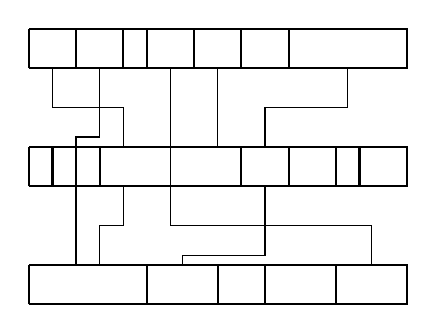
\begin{tikzpicture}
\foreach \y in {0,1,2} {
  \draw[thick] (0,1.5*\y) -- (0,0.5+1.5*\y);
}
\foreach \y/\xa/\xb in {0/0/5,0/5/8,0/8/10,0/10/13,0/13/16,1/0/1,1/1/3,1/3/9,1/9/11,1/11/13,1/13/14,1/14/16,2/0/2,2/2/4,2/4/5,2/5/7,2/7/9,2/9/11,2/11/16} {
  \draw[thick] (0.3*\xa,1.5*\y) -- (0.3*\xb,1.5*\y) -- (0.3*\xb,0.5+1.5*\y) -- (0.3*\xa,0.5+1.5*\y);
}
\foreach \ya/\xa/\ym/\yb/\xb in {2/1/1.5/1/4,2/3/1.25/0/2,2/6/0.5/0/14.5,2/8/1.5/1/8,2/13.5/1.5/1/10,1/4/0.5/0/3,1/10/0.25/0/6.5} {
  \draw (0.3*\xa,1.5*\ya) -- (0.3*\xa,0.25+1.5*\ym) -| (0.3*\xb,0.5+1.5*\yb);
}
\end{tikzpicture}
\caption{Ontwerp met standaard cellen.}
\figlab{standardcells}
\end{figure}
\subsubsection{Gate-array}
Een techniek die nog minder ontwerp-kosten met zich meebrengt is de \termen{Gate Array}. Hierbij beschouwen we een tweedimensionaal rooster van identieke poorten\footnote{Meestal worden hiervoor NAND-poorten gebruikt. Bijvoorbeeld een 3-input NAND-poort.}, de zogenoemde ``\termen{Sea of Gates}''. In dit rooster heeft elke poort identieke afmetingen, en wordt er ruimte gelaten voor bedrading. Opnieuw bevinden zich alle ingangen bovenaan en de uitgangen onderaan. Enkel de bedrading is vervolgens nog uniek aan het product. Dit heeft niet alleen het voordeel van goedkoop ontwerp, de rooster kunnen in massa geproduceerd worden, om daarna elk tot een specifieke circuit uit te groeien. Enkel de metallisatielaag\footnote{De laag waar de verbindingen gelegd worden.} is dus uniek.
\subsection{Programmeerbare chips}
\label{ss:programmeerbareChips}
Prototypes waar nog fouten uitgehaald moeten worden, of elektronica in bijvoorbeeld computers waar de firmware kan veranderen, worden meestal ge\"implementeerd met \termen{programmeerbare chips}. Maar ook onder de programmeerbare chips bestaan nog verschillende technologie\"en. Vooral de programmeertechnieken zijn zeer divers. Hieronder worden de meest courante technieken opgesomd. Vervolgens worden deze technieken verder toegelicht in de subsubsecties.
\begin{itemize}
 \item \termen{Zekeringen}: Hierbij bevat de chip een groot aantal zekeringen. We kunnen dan vervolgens een deel van deze zekeringen doorbranden, om de logica te implementeren. Deze techniek is irreversibel. Immers kan een doorgebrande zekeringen niet hersteld worden. Weliswaar blijft bijprogrammeren\footnote{In een tweede iteratie andere zekeringen doorbranden.} wel mogelijk.%TODO: doorgebrande weglaten?
 \item \termen{Flash-programmeerbaar}: Hierbij kunnen we verbindingen openen en sluiten met transistoren waarbij de gate opgeladen kan worden. Hierdoor wordt herprogrammeren mogelijk, dit is echter traag, en bovendien zal na enige tijd het flash geheugen niet meer herprogrammeerbaar zijn.
 \item \termen{Geheugen-programmeerbaar}: Hierbij bevat de chip een geheugen component, meestal in \termen{SRAM}. De transistoren die de verbindingen bepalen worden dan gekoppeld aan dit geheugen. Het voordeel hierbij is dat we makkelijk en snel de chip kunnen programmeren, en dit kan zelfs dynamisch\footnote{De chip kan tijdens uitvoering zijn gedrag aanpassen.}. Het nadeel is dat dit geheugen telkens bij het aanleggen van voedingsspanning weer opnieuw ingeladen moet worden. Het typevoorbeeld van deze techniek is een \termen{Field Programmable Gate Array (FPGA)}.
\end{itemize}
\subsubsection{Programmable Logic Array (PLA)}
In sectie \ref{s:synthese} zagen we reeds dat we alle logische functies kunnen maken met een \termen{Sum-of-Products (SOP)}. Een \termen{Programmable Logic Array (PLA)} is gebaseerd op dit idee. Deze chip bevat twee rasters van poorten: een \termen{AND-matrix} en een \termen{OR-matrix}. Als ingangen kunnen we vervolgens zowel een variable als zijn inverse aanleggen. \figref{plaSchema}
\begin{figure}[hbt]
\centering
\begin{tikzpicture}[circuit logic US]
\foreach \y in {0,1,...,7} {
  \node[and gate, inputs={normal,normal,normal,normal,normal,normal,normal,normal},scale=0.5] (A\y) at (-1,0.8*\y) {$A\y$};
  \node[or gate, inputs={normal,normal,normal,normal,normal,normal,normal,normal},rotate=-90,scale=0.5] (O\y) at (0.8*\y,-1) {$O\y$};
  \draw (O\y.output) -- ++(0,-0.5) node[scale=0.75,anchor=north]{$f_\y$};
}
\foreach \t/\xa/\xb/\xc/\xd in {0/0/1/8/7,1/2/3/6/5,2/4/5/4/3,3/6/7/2/1} {
  \node[not gate,scale=0.5,rotate=-90] (N\t) at (-6.8+1.6*\t,6.6) {$N\t$};
  \draw[very thin] (N\t.input) |- ++(-0.8,0.5);
  \draw[very thin] (-7.6+1.6*\t,7.6) node[anchor=south,scale=0.75] {$x_\t$} -- (-7.6+1.6*\t,0 |- N\t.output);
  \coordinate (I\xa) at (-7.6+1.6*\t,0 |- N\t.output);
  \coordinate (I\xb) at (N\t.output);
  \draw[very thin] (I\xa) -- (I\xa |- A0.input \xc);
  \draw[very thin] (I\xb) -- (I\xb |- A0.input \xd);
}
\draw[dashed] (-8,-0.9) node[anchor=south west,scale=0.75]{AND-matrix} rectangle (-1.8,6);
\draw[dashed] (-0.4,-0.4) rectangle (6,6.5) node[anchor=north east,scale=0.75]{OR-matrix};
\foreach \y/\yf in {0/8,1/7,2/6,3/5,4/4,5/3,6/2,7/1} {
  \draw[very thin] (A\y.output) -- (O7.input \yf |- A\y.output);
  \foreach \yi/\yid in {1/7,2/6,3/5,4/4,5/3,6/2,7/1,8/0} {
    \draw[very thin] (A\y.input \yi -| I\yid) -- (A\y.input \yi);
    \draw[very thin] (O\y.input \yi) -- (O\y.input \yi |- A\yid.output);
    \fill (O\y.input \yi |- A\yid.output) circle (0.035 cm);
    \fill (A\y.input \yi -| I\yid) circle (0.035 cm);
  }
}
\foreach \y/\x/\xi in {0/0/8,0/2/6,0/4/4,0/7/1,1/0/8,1/2/6,1/4/4,1/6/2,2/1/7,2/2/6,2/5/3,2/6/2,3/1/7,3/2/6,3/5/3,3/6/2,4/0/8,4/3/5,4/5/3,4/7/1,5/0/8,5/2/6,5/4/4,5/7/1,6/0/8,6/2/6,6/5/3,6/7/1,7/1/7,7/3/5,7/4/4,7/6/2,2/3/5,2/4/4,0/6/2} {
  \draw[thick] (A\y.input \xi -| I\x) -- ++(0.05,0.05);
  \draw[thick] (A\y.input \xi -| I\x) -- ++(-0.05,0.05);
  \draw[thick] (A\y.input \xi -| I\x) -- ++(0.05,-0.05);
  \draw[thick] (A\y.input \xi -| I\x) -- ++(-0.05,-0.05);
}

\foreach \y/\x/\xi in {0/1/7,0/2/6,0/3/5,0/5/3,0/7/1,1/1/7,1/2/6,1/3/5,2/0/8,2/2/6,2/3/5,2/5/3,2/7/1,3/0/8,3/5/3,3/6/2,4/1/7,4/2/6,4/4/4,4/7/1,5/1/7,5/2/6,6/2/6,6/4/4,6/5/3,6/6/2,7/0/8,7/5/3,7/7/1} {
  \draw[thick] (O\y.input \xi |- A\x.output) -- ++(0.05,0.05);
  \draw[thick] (O\y.input \xi |- A\x.output) -- ++(-0.05,0.05);
  \draw[thick] (O\y.input \xi |- A\x.output) -- ++(0.05,-0.05);
  \draw[thick] (O\y.input \xi |- A\x.output) -- ++(-0.05,-0.05);
}
\end{tikzpicture}
\caption{Schematische voorstelling van een Programmable Logic Array (PLA).}
\figlab{plaSchema}
\end{figure}
toont een schematische voorstelling van zo'n PLA. De punten tussen twee verbindingen stellen een zekering door. Door zekeringen door te branden kunnen we dus het model aanpassen. Punten waar een kruisje bij staat zijn in dit voorbeeld doorgebrand. Bij een doorgebrande zekering in de AND-matrix, komt er een 1 op de lijn, bij een doorgebrande zekering op de OR-matrix een 0. Er bestaan nog twee varianten op een PLA:
\begin{itemize}
 \item een \termen{Programmable Array Logic (PAL)} heeft een vaste OR-matrix.
 \item een \termen{Programmable Read Only Memory (PROM)} heeft een vaste AND-matrix. Hierbij fungeert deze matrix als een adresdecoder (zie \ref{ss:decoder}).
\end{itemize}
\subsubsection{Programmable Logic Device (PLD)}
\label{sss:pld}
Een PLA is niet in staat complexe functies te beschrijven zonder de AND- en OR-matrix zeer groot te maken. Omdat immers voor iedere verbinding ook nog lijnen moeten voorzien worden, zou de component al snel te groot worden. Een \termen{Programmable Logic Device (PLD)} probeert hierop een antwoord te bieden. Hierbij wordt meer lagen logica gehanteerd. \figref{pldSchema}
\begin{figure}[hbt]
\centering
\begin{tikzpicture}[circuit logic US] %yscale=0.8
\foreach\y/\ia/\ib in {0/1/2,1/3/4,2/5/6,3/7/8,4/9/10} {
  \node[not gate,scale=0.5] (N\y) at (0,\y) {$N\y$};
  \coordinate (I\y) at (-1-0.1*\y,0.5+\y);
  \draw[very thin] (I\y) -- (-0.5,0.5+\y -| N\y.output);
  \draw[very thin] (N\y) -| ++(-0.5,0.5);
  \coordinate (B\ia) at (N\y.output);
  \coordinate (B\ib) at (N\y.output |- -0.5,0.5+\y);
}
\draw (I3) node[anchor=east,scale=0.75]{$x_1$};
\draw (I4) node[anchor=east,scale=0.75]{$x_2$};
\foreach\s in {0,1,...,3} {
  \node[or gate,inputs={normal,normal,normal,normal,normal},scale=0.5,rotate=-90] (O\s) at (3*\s+2.2,-2) {};
  \foreach\x/\xi/\iy in {0/5/0.7,1/4/0.6,2/3/0.5,3/2/0.6,4/1/0.7} {
    \node[and gate,inputs={normal,normal,normal,normal,normal,normal,normal,normal,normal,normal},scale=0.333,rotate=-90] (A\s\x) at (3*\s+0.6*\x+1,-1) {};
    \draw[very thin] (A\s\x.output) -- ++(0,-\iy+0.5) -| (O\s.input \xi);
    \foreach \g in {1,2,...,10} {
      \fill (B\g -| A\s\x.input \g) circle (0.035 cm);
      \draw[very thin] (B\g -| A\s\x.input \g) -- (A\s\x.input \g);
    }
  }
}
\foreach\s in {0,3} {
  \coordinate (OO\s) at (O\s.output |- 0,-3-0.1*\s);
  \coordinate (OOO\s) at (OO\s);
  \draw (O\s.output) -- (OO\s);
}
\foreach\s in {1,2} {
  \node[draw=black,rectangle] (D\s) at (3*\s+2.8,-3.125) {D};
  \draw[very tiny] (D\s.north) |- ++(-0.6,0.25);
  \coordinate (OO\s) at (3*\s+2.5,-4.5-0.1*\s);
  \draw[very tiny] (D\s.south) -- (D\s.south |- 0,-3.75);
  \draw[very thin] (O\s.output) -- (O\s.output |- 0,-3.75);
  \draw[very thin] (3*\s+2.5,-4.25) -- (OO\s);
  \coordinate (OOO\s) at (OO\s |- 0,-5.5);
  \draw[very thin] (OO\s) -- (OOO\s);
  \draw (3*\s+2,-3.75) -- (3*\s+3,-3.75) -- (3*\s+2.8,-4.25) -- (3*\s+2.2,-4.25) -- cycle;
}
\foreach\s in {0,1,...,2} {
  \draw[very thin] (OO\s) -| (I\s);
}
\foreach\s in {1,2,3} {
  \draw(OOO\s) node[anchor=north,scale=0.75] {$f_\s$};
}
\foreach\y in {1,2,...,10} {
  \draw[very thin] (B\y) -- (B\y -| A34.input \y);
}
\foreach \s/\x/\g in {0/0/1,0/0/2,0/0/3,0/0/4,0/0/6,0/0/7,0/0/10,0/1/1,0/1/3,0/1/4,0/1/5,0/1/6,0/1/8,0/1/10,0/2/1,0/2/2,0/2/3,0/2/4,0/2/6,0/2/8,0/2/10,0/3/1,0/3/2,0/3/3,0/3/6,0/3/7,0/3/9,0/3/10,0/4/1,0/4/3,0/4/5,0/4/6,0/4/7,0/4/10,1/0/1,1/0/2,1/0/4,1/0/6,1/0/7,1/0/9,1/0/10,1/1/2,1/1/4,1/1/6,1/1/8,1/1/9,1/1/10,1/2/1,1/2/2,1/2/3,1/2/6,1/2/7,1/2/8,1/2/9,1/3/1,1/3/3,1/3/4,1/3/6,1/3/7,1/3/8,1/3/10,1/4/1,1/4/2,1/4/3,1/4/4,1/4/5,1/4/7,1/4/9,1/4/10,2/0/2,2/0/3,2/0/4,2/0/6,2/0/7,2/0/8,2/0/10,2/1/2,2/1/4,2/1/5,2/1/6,2/1/8,2/1/9,2/1/10,2/2/1,2/2/2,2/2/3,2/2/5,2/2/6,2/2/7,2/2/8,2/2/10,2/3/1,2/3/2,2/3/3,2/3/5,2/3/7,2/3/8,2/3/9,2/3/10,3/4/1,3/4/3,3/4/4,3/4/6,3/4/8,3/4/10,3/0/2,3/0/3,3/0/4,3/0/6,3/0/7,3/0/8,3/0/9,3/1/2,3/1/3,3/1/6,3/1/7,3/1/9,3/2/1,3/2/2,3/2/4,3/2/5,3/2/7,3/2/10,3/3/1,3/3/2,3/3/3,3/3/4,3/3/6,3/3/8,3/3/9,3/4/2,3/4/4,3/4/6,3/4/7,3/4/9} {
  \draw[thick] (B\g -| A\s\x.input \g) -- ++(0.05,0.05);
  \draw[thick] (B\g -| A\s\x.input \g) -- ++(-0.05,0.05);
  \draw[thick] (B\g -| A\s\x.input \g) -- ++(0.05,-0.05);
  \draw[thick] (B\g -| A\s\x.input \g) -- ++(-0.05,-0.05);
}
\end{tikzpicture}%TODO: make more compact + multiplexer input
\caption{Schematische voorstelling van een Programmable Logic Device (PLD).??}
\figlab{pldSchema}
\end{figure}
toont het idee achter deze techniek. We beschouwen nog steeds een matrix, alleen is een groot deel van de invoer eigenlijk de uitvoer van andere geprogrammeerde functies. Zo zijn $x_1$ en $x_2$ de enig invoerlijnen, de andere lijnen zijn het resultaat van geprogrammeerde logica. Op de figuur bemerken we verder nog dat er componenten onder de uitgangen staan. Deze componenten komen later in de cursus aan bod. Het vierkant stelt een 1-bit geheugen voor (zie \ref{s:memory}), meestal een D-Flip Flop. De trapezium een multiplexer (zie \ref{ss:multiplexer}). Dit component laat ons dus toe complexere schakelingen te maken, en tegelijk het aantal zekeringen onder controle te houden.
\subsubsection{Complex Programmable Logic Device (CPLD)}
\begin{figure}[H]%TODO: check alignment, fixed floating environment used [H]
\centering
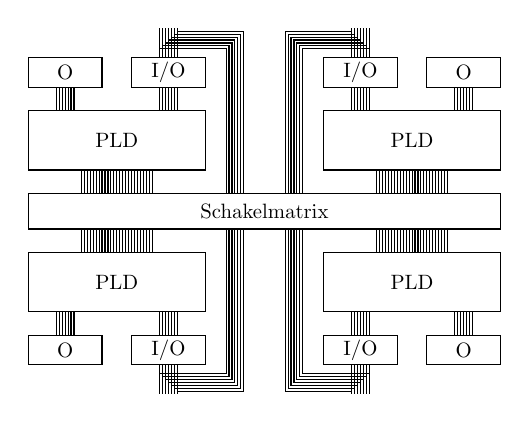
\begin{tikzpicture}[scale=0.75]
\draw (-3.375,-2.35) node[scale=0.75]{O};
\draw (-4,-2.6) rectangle (-2.75,-2.1);
\draw (-1.625,-2.35) node[scale=0.75]{I/O};
\draw (-1,-2.6) rectangle (-2.25,-2.1);
\draw (-2.5,-1.2) node[scale=0.75]{PLD};
\draw (-4,-1.7) rectangle (-1,-0.7);

\draw (3.375,-2.35) node[scale=0.75]{O};
\draw (4,-2.6) rectangle (2.75,-2.1);
\draw (1.625,-2.35) node[scale=0.75]{I/O};
\draw (1,-2.6) rectangle (2.25,-2.1);
\draw (2.5,-1.2) node[scale=0.75]{PLD};
\draw (4,-1.7) rectangle (1,-0.7);

\draw (-3.375,2.35) node[scale=0.75]{O};
\draw (-4,2.6) rectangle (-2.75,2.1);
\draw (-1.625,2.35) node[scale=0.75]{I/O};
\draw (-1,2.6) rectangle (-2.25,2.1);
\draw (-2.5,1.2) node[scale=0.75]{PLD};
\draw (-4,1.7) rectangle (-1,0.7);

\draw (3.375,2.35) node[scale=0.75]{O};
\draw (4,2.6) rectangle (2.75,2.1);
\draw (1.625,2.35) node[scale=0.75]{I/O};
\draw (1,2.6) rectangle (2.25,2.1);
\draw (2.5,1.2) node[scale=0.75]{PLD};
\draw (4,1.7) rectangle (1,0.7);
\draw (0,0) node[scale=0.75]{Schakelmatrix};
\draw (-4,-0.3) rectangle (4,0.3);
\foreach \x in {-3,-2,...,3} {
  \draw (-3.375+0.05*\x,-2.1) -- (-3.375+0.05*\x,-1.7);
  \draw (-1.625+0.05*\x,-2.1) -- (-1.625+0.05*\x,-1.7);
  \draw (-1.625+0.05*\x,-2.6) -- (-1.625+0.05*\x,-3.1);

  \draw (3.375+0.05*\x,-2.1) -- (3.375+0.05*\x,-1.7);
  \draw (1.625+0.05*\x,-2.1) -- (1.625+0.05*\x,-1.7);
  \draw (1.625+0.05*\x,-2.6) -- (1.625+0.05*\x,-3.1);

  \draw (-3.375+0.05*\x,2.1) -- (-3.375+0.05*\x,1.7);
  \draw (-1.625+0.05*\x,2.1) -- (-1.625+0.05*\x,1.7);
  \draw (-1.625+0.05*\x,2.6) -- (-1.625+0.05*\x,3.1);

  \draw (3.375+0.05*\x,2.1) -- (3.375+0.05*\x,1.7);
  \draw (1.625+0.05*\x,2.1) -- (1.625+0.05*\x,1.7);
  \draw (1.625+0.05*\x,2.6) -- (1.625+0.05*\x,3.1);
  
  \draw (-0.5+0.05*\x,0.3) |- (-1.625+0.05*\x,2.9+0.05*\x);
  \draw (0.5-0.05*\x,0.3) |- (1.625-0.05*\x,2.9+0.05*\x);
  \draw (-0.5+0.05*\x,-0.3) |- (-1.625+0.05*\x,-2.9-0.05*\x);
  \draw (0.5-0.05*\x,-0.3) |- (1.625-0.05*\x,-2.9-0.05*\x);
}
\foreach \x in {-12,-11,...,12} {
  \draw (-2.5-0.05*\x,-0.7) -- (-2.5-0.05*\x,-0.3);
  \draw (-2.5-0.05*\x,0.7) -- (-2.5-0.05*\x,0.3);
  \draw (2.5-0.05*\x,-0.7) -- (2.5-0.05*\x,-0.3);
  \draw (2.5-0.05*\x,0.7) -- (2.5-0.05*\x,0.3);
}
\end{tikzpicture}
\caption{Schematische voorstelling van een Complex Programmable Logic Device (CPLD).}
\figlab{cpldSchema}
\end{figure}
Een aantal PLD componenten samen op \'e\'en chip samen met de zogenaamde \termen{Glue Logic} om ze samen te laten werken, noemen we een \termen{Complex Programmable Logic Device (CPLD)}. \figref{cpldSchema} toont dat deze glue eigenlijk neerkomt op een \termen{schakelmatrix} om PLDs te laten samenwerken en \termen{in- en uitvoer modules} om te intrageren met de buitenwereld. Naast de PLDs zelf dient dus ook de schakelmatrix geprogrammeerd te worden. Een ander belangrijk verschil is dat CPLDs niet geprogrammeerd worden met behup van zekeringen. De chip wordt geprogrammeerd door ladingen op transistoren te plaatsen, bijgevolg kunnen de we deze chip enkele keren volledig herprogrammeren.
\subsubsection{Field Programmable Gate Array (FPGA)}
Een nog meer geavanceerde programmeerbare chip is de \termen{Field Programmable Gate Array (FPGA)}. Net zoals bij een CPLD bevat deze chip enkele logische blokken met daartussen ``glue''. Deze ``glue'' uit zich opnieuw in een schakelmatrix, maar ook in korte en lange verbindingen. Deze laatsten worden vaak ook \termen{lange lijnen} genoemd. Daarnaast bevat de chip uiteraard ook opnieuw en- en uitvoer modulen. \figref{fpgaSchemaFull}
\begin{figure}[hbt]
\centering
\subfigure[Volledige FPGA]{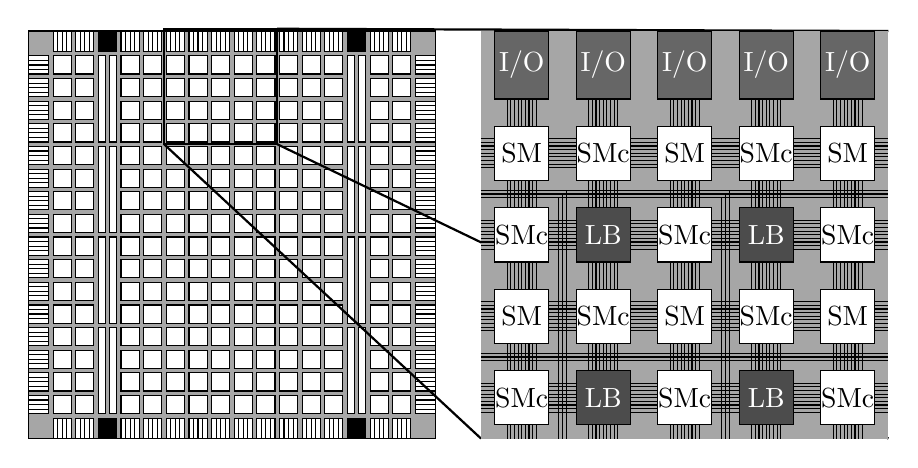
\begin{tikzpicture}[scale=1.15]
\filldraw[fill=black!35,draw=black] (0,0) rectangle (4.5,4.5);
\foreach \y in {1,2,...,16} {
  \fill[fill=white,draw=black] (0.25*\y+0.025,0) rectangle ++(0.20,0.225);
  \fill[fill=white,draw=black] (0.25*\y+0.025,4.275) rectangle ++(0.20,0.225);
  \fill[fill=white,draw=black] (0,0.25*\y+0.025) rectangle ++(0.225,0.20);
  \fill[fill=white,draw=black] (4.275,0.25*\y+0.025) rectangle ++(0.225,0.20);
  \foreach \xs in {1,2,3} {
    \draw (0.25*\y+0.05*\xs+0.025,0) -- ++(0,0.225);
    \draw (0.25*\y+0.05*\xs+0.025,4.275) -- ++(0,0.225);
  \draw (0,0.25*\y+0.05*\xs+0.025) -- ++(0.225,0);
    \draw (4.275,0.25*\y+0.05*\xs+0.025) -- ++(0.225,0);
  }
  \foreach \x in {1,2,4,5,...,13,15,16} {
    \filldraw[fill=white,draw=black] (0.25*\x+0.025,0.25*\y+0.025) rectangle ++(0.20,0.20);
  }
}
\foreach \x in {3,14} {
  \fill (0.25*\x+0.025,0) rectangle ++(0.20,0.225);
  \fill (0.25*\x+0.025,4.275) rectangle ++(0.20,0.225);
  \foreach \y in {0,1,...,3} {
    \filldraw[fill=white,draw=black] (0.25*\x+0.025,\y+0.275) rectangle ++(0.075,0.95);
    \filldraw[fill=white,draw=black] (0.25*\x+0.15,\y+0.275) rectangle ++(0.075,0.95);
  }
}
\draw[thick] (1.5,4.525) rectangle ++(1.25,-1.275);
\begin{scope}[xshift=5 cm]
\draw[thick] (-3.5,3.25) -- (0,0);
\draw[thick] (-2.25,3.25) -- (4.5,0);
\draw[thick] (-2.25,4.525) -- (4.5,4.5);
\fill[fill=black!35] (0,0) rectangle (4.5,4.5);
\foreach \x in {0,1,...,4} {
  \filldraw[fill=black!60,draw=black] (0.9*\x+0.15,3.75) rectangle ++(0.6,0.75);
  \draw (0.9*\x+0.45,4.125) node[white] {I/O};
}
\foreach \x in {0,2,4} {
  \foreach \y in {1,3} {
    \filldraw[fill=white,draw=black] (0.9*\x+0.15,0.9*\y+0.15) rectangle ++(0.6,0.6);
    \draw (0.9*\x+0.45,0.9*\y+0.45) node{SM};
  }
  \foreach \y in {0,2} {
    \filldraw[fill=white,draw=black] (0.9*\x+0.15,0.9*\y+0.15) rectangle ++(0.6,0.6);
    \draw (0.9*\x+0.45,0.9*\y+0.45) node{SMc};
  }
}
\foreach \x in {1,3} {
  \foreach \y in {0,2} {
    \filldraw[fill=black!70,draw=black] (0.9*\x+0.15,0.9*\y+0.15) rectangle ++(0.6,0.6);
    \draw (0.9*\x+0.45,0.9*\y+0.45) node[white]{LB};
  }
  \foreach \y in {1,3} {
    \filldraw[fill=white,draw=black] (0.9*\x+0.15,0.9*\y+0.15) rectangle ++(0.6,0.6);
    \draw (0.9*\x+0.45,0.9*\y+0.45) node{SMc};
  }
}
\foreach \y in {0,1,...,3} {
  \foreach \s in {-4,-3,...,4} {
    \draw (0,0.9*\y+0.45+0.04*\s) -- ++(0.15,0);
    \draw (4.35,0.9*\y+0.45+0.04*\s) -- ++(0.15,0);
    \foreach \x in {0,1,...,4} {
      \draw (0.9*\x+0.45+0.04*\s,0.9*\y+0.75) -- ++(0,0.3);
    }
    \foreach \x in {0,1,...,3} {
      \draw (0.9*\x+0.75,0.9*\y+0.45+0.04*\s) -- ++(0.3,0);
    }
  }
}
\foreach \x in {0,1,...,4} {
  \foreach \s in {-4,-3,...,4} {
    \draw (0.9*\x+0.45+0.04*\s,0) -- ++(0,0.15);
  }
}
\foreach \s in {-1,0,1} {
  \foreach \y in {0,2} {
    \draw (0,0.9*\y+0.04*\s+0.9) -- ++(4.5,0);
    \draw (0.9*\y+0.04*\s+0.9,0) -- ++(0,0.04*\s+2.7);
  }
}
\end{scope}
\end{tikzpicture}
\figlab{fpgaSchemaFull}}
\subfigure[Logical Block (LB)] {
\begin{tikzpicture}
\filldraw[fill=black!35,draw=black] (-0.5,-0.5) rectangle (3.5,2.5);
\filldraw[fill=white,draw=black] (0.1,0.1) rectangle ++(1.8,1.8);
\filldraw[fill=white,draw=black] (2.9,0.8) rectangle ++(-0.7,0.4);
\draw (1.9,1) -- (2.2,1);
\draw (2.05,1) |- (4,1.5) node[anchor=west,scale=0.7]{$y$};
\draw (2.9,1) -- (4,1) node[anchor=west,scale=0.7]{$y_Q$};
\draw (2.55,1) node[scale=0.7]{D-FF};
\draw (1,1) node[alignment=center,text width=2 cm,scale=0.7] {$16\times1$ LUT: logische functie van 4 variabelen};
\foreach \y/\yt in {-2/4,-1/3,0/2,1/1} {
  \draw (-1,1.2+0.4*\y) node[anchor=east,scale=0.7]{$x_\yt$} -- ++(1.1,0);
}
\end{tikzpicture}
\figlab{fpgaSchemaLB}}
\subfigure[Schakelmatrix]{
\begin{tikzpicture}
\filldraw[fill=black!35,draw=black] (0,0) rectangle (3,3);
\node[nmoso,rotate=-90,scale=0.8] (N1) at (0.75,2.5) {};
\node[nmosc,rotate=-90,scale=0.8] (N2) at (2.25,2.5) {};
\node[nmosc,scale=0.8] (N3) at (1.5,2) {};
\node[nmoso,rotate=-90,scale=0.8] (N4) at (2,1.5) {};
\node[nmoso,rotate=-90,scale=0.8] (N5) at (0.75,0.5) {};
\node[nmoso,rotate=-90,scale=0.8] (N6) at (2.25,0.5) {};
\draw (N2.drain) -- (N2.drain -| 2.75,0) |- (N6.drain);
\draw (N1.drain) -- (N2.source);
\draw (N1.source) -- (N1.source -| 0.25,0) |- (N5.source);
\draw (N5.drain) -- (N6.source);
\draw (N4.source) -- (-0.5,1.5);
\draw (N4.drain) -- (3.5,1.5);
\draw (N3.source) -- (1.5,-0.5);
\draw (N3.drain) -- (1.5,3.5);
\fill (N4.source -| 0.25,0) circle (0.035 cm);
\fill (N4.drain -| 2.75,0) circle (0.035 cm);
\fill (N3.source |- N1.source) circle (0.035 cm);
\fill (N3.drain |- N6.source) circle (0.035 cm);
\end{tikzpicture}
\figlab{fpgaSchemaSchakelMatrix}
}
\caption{Schematische voorstelling van een Field Programmable Gate Array (FPGA).}
\figlab{fpgaSchema}
\end{figure}
schematiseert dit concept. In tegenstelling tot een CPLD heeft een FPGA andere logische bouwblokken, namelijk \termen{Logical Blocks (LB)}. Dit logische blok staat weergegeven op \figref{fpgaSchemaLB}. Het bestaat typisch uit 4 ingangen ($x_1$, $x_2$, $x_3$ en $x_4$) en twee uitgangen ($y$ en $y_Q$). Inwendig bestaat het uit een 16 bit \termen{Look-Up Table (LUT)} en een \termen{Data Flip-Flop (D-FF)}. Deze Look-Up Table is in feite niets anders dan een klein geheugen. Met de 4 ingangen zijn we in staat om 16 verschillende invoer-waarden te genereren. Voor elk van deze waarden programmeren we een bit als uitvoer. Deze wordt uitgevoerd langs de $y$. De Data Flip-Flop houdt deze bit 1 klokcyclus bij, en zal hem de volgende klokcyclus op $y_Q$ zetten. Het gevolg is dus dat $y_Q$ een klokflank na-ijlt op $y$. Tot slot beschouwen we op \figref{fpgaSchemaSchakelMatrix} de implementatie van een \termen{schakelmatrix}. Hierbij verbinden we 4 lijnen met elkaar. Dit levert dus 6 mogelijke verbindingen. Door het programmeren van de chip, kunnen we de transistoren openen of sluiten, wat resulteert in het al dan niet verbinden van twee verbindingen. De transistoren die men hierbij gebruikt zijn de zogenaamde ``\termen{Pass-transistoren}''.
\paragraph{Spartan-3}
Een beroemde FPGA-chip is de \termen{Spartan-3} van \emph{Xilinx}. Deze FPGA maakt gebruik van \termen{Configurable Logic Blocks (CLB)} in plaats van LBs. Een CLB wordt onderverdeeld in 4 ``\termen{slices}''. Twee van deze slices kunnen geconfigureerd worden als schuifregisters (zie \ref{s:schuifregisters}), geheugencellen, of logische blokken, de overige twee alleen als logische blokken. Deze complexere slices bevatten twee verschillende componenten voor logica: 2 functies met 4 variabelen, en 1 functie met 5 variabelen, meestal aangevuld met flipflops. Verder bevatten deze vaak een multiplexer en een schuifregister. De specificaties van deze slices zijn verder ook terug te vinden in \cite[p.~22-23]{xilinxFpgaDs099}. Verder zien we op \figref{fpgaSchemaFull} ook dat er naast logische en in- en uitvoer blokken ook nog andere componenten op een FPGA zitten. Meestal gaat het dan om RAM en een multiplexer. Bovendien bevat de chip ook enkele klokken die het systeem aansturen. Deze zijn als een zwart blokje weergegeven. Typische frequenties bevinden zich rond de 50 MHz. Modernere FPGA's uiten zich in grotere geheugens, soms zelfs met een Stack (LIFO, zie \sscref{stack}), specifieke in- en uitvoer blokken zoals Ethernet, PCIe,... tot zelfs microprocessoren.
\section{Praktische aspecten}
Tot nu toe hebben we ons bezig gehouden met de implementatie van chips. Deze implementatie hebben we afgeleid uit de circuits. Er zijn echter ook aspecten die een invloed hebben op de werking die niet altijd van het circuit kunnen afgelezen worden. Zoals bijvoorbeeld de geometrie van de chip. De volgende subsecties beschrijven met welke praktische aspecten rekening gehouden moeten worden bij het ontwerpen.
\subsection{Spanningsniveaus en ruismarge}
\subsubsection{Ruismarge}
In sectie \ref{s:logischeWaarden} hebben we reeds kort beschreven dat we een bereik specificeren voor een \termen{High} en \termen{Low} signaal.  We definieerden ook een ongedefinieerde zone. Deze zone wordt gebruikt indien het onduidelijk wordt wat er precies aan de ingang staat. Uiteraard willen we vermijden dat we ooit in deze ruismarge terecht komen. Daarom introduceren we een \termen{Ruismarge}. Dit is een spanningsmarge die we beschikbaar stellen door een kleiner gebied van uitgangsspanningen te gebruiken dan toegelaten. We zullen dus de poorten spanningen laten genereren die zich in het hoogste gedeelte van High bevinden, of in het laagste gedeelte van Low. De ruis zal het signaal uiteraard kunnen afzwakken, maar we bijven in de acceptabele zone van High en Low. Het resultaat is dus dat bij de marges van de ingangen ruimer is dan de marges van de uitgangen. \figref{noiseMargin} geeft dit concept schematisch weer. Ook vermeldt de figuur de typische spanningsniveaus bij CMOS en TTL\footnote{TTL: Transistor-Transistor Logic.} implementatie.
\begin{figure}[hbt]
\centering
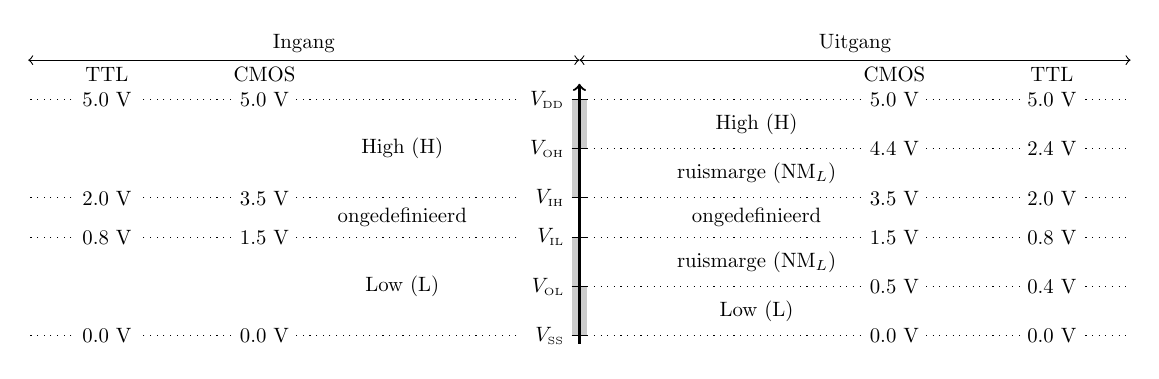
\begin{tikzpicture}
\fill[black!20] (-0.1,0) rectangle (0,1.25);
\fill[black!20] (-0.1,1.75) rectangle (0,3);
\fill[black!20] (0,0.625) rectangle (0.1,0);
\fill[black!20] (0,2.375) rectangle (0.1,3);
\draw[thick,->] (0,-0.1) -- (0,3.2);
\draw (-0.1,0) node[anchor=east,scale=0.75]{$V_{\mbox{\tiny SS}}$} -- (0.1,0);
\draw (-0.1,0.625) node[anchor=east,scale=0.75]{$V_{\mbox{\tiny OL}}$} -- (0.1,0.625);
\draw (-0.1,1.25) node[anchor=east,scale=0.75]{$V_{\mbox{\tiny IL}}$} -- (0.1,1.25);
\draw (-0.1,1.75) node[anchor=east,scale=0.75]{$V_{\mbox{\tiny IH}}$} -- (0.1,1.75);
\draw (-0.1,2.375) node[anchor=east,scale=0.75]{$V_{\mbox{\tiny OH}}$} -- (0.1,2.375);
\draw (-0.1,3) node[anchor=east,scale=0.75]{$V_{\mbox{\tiny DD}}$} -- (0.1,3);
\draw[<->] (-7,3.5) to node[midway,above,scale=0.75]{Ingang} (0,3.5);
\draw[<->] (7,3.5)  to node[midway,above,scale=0.75]{Uitgang} (0,3.5);

\draw (4,3.5) node[anchor=north,scale=0.75]{CMOS};
\draw (6,3.5) node[anchor=north,scale=0.75]{TTL};
\draw (-4,3.5) node[anchor=north,scale=0.75]{CMOS};
\draw (-6,3.5) node[anchor=north,scale=0.75]{TTL};
\draw (2.25,1.5) node[scale=0.75]{ongedefinieerd};
\draw (-2.25,1.5) node[scale=0.75]{ongedefinieerd};
\draw (2.25,2.6875) node[scale=0.75]{High (H)};
\draw (2.25,0.3125) node[scale=0.75]{Low (L)};
\draw (2.25,0.9375) node[scale=0.75]{ruismarge (NM$_L$)};
\draw (2.25,2.0625) node[scale=0.75]{ruismarge (NM$_L$)};
\draw (-2.25,2.375) node[scale=0.75]{High (H)};
\draw (-2.25,0.625) node[scale=0.75]{Low (L)};

\draw[dotted] (0.1,3) -- ++(6.9,0);
\draw[dotted] (0.1,2.375) -- ++(6.9,0);
\draw[dotted] (0.1,1.75) -- ++(6.9,0);
\draw[dotted] (0.1,1.25) -- ++(6.9,0);
\draw[dotted] (0.1,0.625) -- ++(6.9,0);
\draw[dotted] (0.1,0) -- ++(6.9,0);

\draw[dotted] (-0.8,3) -- ++(-6.2,0);
\draw[dotted] (-0.8,1.75) -- ++(-6.2,0);
\draw[dotted] (-0.8,1.25) -- ++(-6.2,0);
\draw[dotted] (-0.8,0) -- ++(-6.2,0);

\filldraw[fill=white,draw=black] (4,3) node[scale=0.75,fill=white]{5.0 V};
\filldraw[fill=white,draw=black] (4,2.375) node[scale=0.75,fill=white]{4.4 V};
\filldraw[fill=white,draw=black] (4,1.75) node[scale=0.75,fill=white]{3.5 V};
\filldraw[fill=white,draw=black] (4,1.25) node[scale=0.75,fill=white]{1.5 V};
\filldraw[fill=white,draw=black] (4,0.625) node[scale=0.75,fill=white]{0.5 V};
\filldraw[fill=white,draw=black] (4,0) node[scale=0.75,fill=white]{0.0 V};
\filldraw[fill=white,draw=black] (6,3) node[scale=0.75,fill=white]{5.0 V};
\filldraw[fill=white,draw=black] (6,2.375) node[scale=0.75,fill=white]{2.4 V};
\filldraw[fill=white,draw=black] (6,1.75) node[scale=0.75,fill=white]{2.0 V};
\filldraw[fill=white,draw=black] (6,1.25) node[scale=0.75,fill=white]{0.8 V};
\filldraw[fill=white,draw=black] (6,0.625) node[scale=0.75,fill=white]{0.4 V};
\filldraw[fill=white,draw=black] (6,0) node[scale=0.75,fill=white]{0.0 V};

\filldraw[fill=white,draw=black] (-4,3) node[scale=0.75,fill=white]{5.0 V};
\filldraw[fill=white,draw=black] (-4,1.75) node[scale=0.75,fill=white]{3.5 V};
\filldraw[fill=white,draw=black] (-4,1.25) node[scale=0.75,fill=white]{1.5 V};
\filldraw[fill=white,draw=black] (-4,0) node[scale=0.75,fill=white]{0.0 V};
\filldraw[fill=white,draw=black] (-6,3) node[scale=0.75,fill=white]{5.0 V};
\filldraw[fill=white,draw=black] (-6,1.75) node[scale=0.75,fill=white]{2.0 V};
\filldraw[fill=white,draw=black] (-6,1.25) node[scale=0.75,fill=white]{0.8 V};
\filldraw[fill=white,draw=black] (-6,0) node[scale=0.75,fill=white]{0.0 V};
\end{tikzpicture}
\caption{Werking van ruismarge bij CMOS en TTL.}
\figlab{noiseMargin}
\end{figure}
\paragraph{Onlogische Spanningen}
Wanneer een transistor omschakelt, betekent dit niet dat van het ene moment op het andere er een andere spanning op de uitgang komt te staan, Deze overgang is een continue proces. Dit betekent dus dat op een zeker moment aan de uitgang de spanning in het ongedefinieerde gebied komt te liggen. Ideaal zou uiteraard zijn dat bij een continue verandering aan de ingang er toch een discrete verandering aan de uitgang plaatsvindt. Dit is echter fysisch onmogelijk. De ontwerper dient dus rekening te houden met dit overgangsverschijnsel. Dit vormt bovendien een groot probleem omdat op dat moment beide transistoren\footnote{PMOS en NMOS.} halfopen zijn, en er dus stroom door de componenten vloeit. Verder weet men ook niet altijd welke spanning er aan de uitgang zal staan. De \termen{Transferfunctie} is immers afhankelijk van zowel het productieproces als omgevingsfactoren zoals warmte,... \figref{transferFunctionMOS} toont verschillende realistische transferfuncties samen met de ideale transferfunctie.
\begin{figure}[hbt]
\centering
\subfigure[Transferfuncties bij een inverter]{
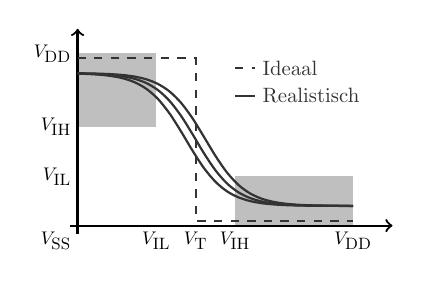
\begin{tikzpicture}
\def\sxy{0.625};
\fill[gray!50] (0,\sxy*2) rectangle ++(1,\sxy*1.5);
\fill[gray!50] (2,0) rectangle ++(1.5,\sxy);
\draw (0,0) node[anchor=north east,scale=0.66]{$V_{\mbox{\small{SS}}}$};
\foreach\x/\t in {1/IL,2/IH,3.5/DD} {
  \draw (\x,0) node[anchor=north,scale=0.66]{$V_{\mbox{\small{\t}}}$};
  \draw (0,\sxy*\x) node[anchor=east,scale=0.66]{$V_{\mbox{\small{\t}}}$};
}
\draw (1.5,0) node[anchor=north,scale=0.66]{$V_{\mbox{\small{T}}}$};
\draw[thick,->] (-0.1,0) -- (4,0);
\draw[thick,->] (0,-0.1) -- (0,2.5);
\draw[thick,dashed,black!80] (2,2) -- (2.25,2) node[anchor=west,scale=0.75]{Ideaal};
\draw[thick,black!80] (2,1.65) -- (2.25,1.65) node[anchor=west,scale=0.75]{Realistisch};
\draw[thick,dashed,black!80] (0,\sxy*3.4) -| (1.5,0.1*\sxy) -- (3.5,0.1*\sxy);
\draw[thick,black!80,variable=\x,domain=0:3.5,smooth] plot (\x,{2.7*\sxy/(1.0+exp(4*\x-6.5))+0.4*\sxy});
\draw[thick,black!80,variable=\x,domain=0:3.5,smooth] plot (\x,{2.7*\sxy/(1.0+exp(4*\x-6))+0.4*\sxy});
\draw[thick,black!80,variable=\x,domain=0:3.5,smooth] plot (\x,{2.7*\sxy/(1.0+exp(4*\x-5.5))+0.4*\sxy});
\end{tikzpicture}
\figlab{transferFunctionMOS}
}
\subfigure[Schmitt-Trigger transferfunctie]{
\begin{tikzpicture}[circuit logic US]
\def\sxy{0.625};
\fill[gray!50] (0,\sxy*2) rectangle ++(1,\sxy*1.5);
\fill[gray!50] (2,0) rectangle ++(1.5,\sxy);
\draw (0,0) node[anchor=north east,scale=0.66]{$V_{\mbox{\small{SS}}}$};
\foreach\x/\t in {1/IL,2/IH,3.5/DD} {
  \draw (\x,0) node[anchor=north,scale=0.66]{$V_{\mbox{\small{\t}}}$};
  \draw (0,\sxy*\x) node[anchor=east,scale=0.66]{$V_{\mbox{\small{\t}}}$};
}
\draw[thick,->] (-0.1,0) -- (4,0);
\draw[thick,->] (0,-0.1) -- (0,2.5);
\draw[thick,black!80,variable=\x,domain=0:3.5,smooth] plot (\x,{2.7*\sxy/(1.0+exp(4*\x-6.5))+0.4*\sxy});
\draw[thick,black!80,variable=\x,domain=0:3.5,smooth] plot (\x,{2.7*\sxy/(1.0+exp(4*\x-4.5))+0.4*\sxy});
\draw[thick,black!80,->] (1.625-0.05,1.75*\sxy+2.7*\sxy*0.05) -- (1.625,1.75*\sxy);
\draw[thick,black!80,->] (1.125+0.05,1.75*\sxy-2.7*\sxy*0.05) -- (1.125,1.75*\sxy);
\node[not gate,scale=0.75] (N) at (2.5,1.75) {};
\draw (N.input) -- ++(-0.25,0);
\draw (N.output) -- ++(0.25,0);
\begin{scope}[xshift=2.5 cm,yshift=1.75 cm,scale=0.6]
\draw (-0.1875,-0.125) -| (0.0625,0.125) -- (0.1875,0.125);
\draw (-0.0625,-0.125) |- (0.0625,0.125);
\end{scope}
\end{tikzpicture}
\figlab{transferFunctionSchmittTrigger}
}
\caption{Transferfuncties en Schmitt-Trigger ingangen.}
\figlab{transferSchmittTrigger}
\end{figure}
\paragraph{Schmitt-trigger ingangen} Dit effect is vooral nadelig voor bijvoorbeeld in- en uitvoer. Deze signalen veranderen doorgaans traag, en bovendien niet strikt stijgend of dalend. Dit heeft tot gevolg dat indien het ingangssignaal van een 0 naar een 1 moet gaan, het meestal verschillende malen van signaal verandert. Een oplossing hiervoor zijn \termen{Schmitt-trigger ingangen}, dit zijn componenten met een \termen{hysteresis}. Dit betekent dat de overgangsspanning bij een overgang van laag naar hoog, hoger is dan de overgangsspanning van hoog naar laag. Deze transferfunctie staat op \figref{transferFunctionSchmittTrigger}, samen met het symbool voor een Schmitt-Trigger ingang: een NOT poort, met een miniatuur van de inverse transferfunctie.
\subsection{Dynamisch gedrag}
\begin{figure}[hbt]
\centering
\begin{tikzpicture}[circuit logic US,american resistors]
\node[not gate] (N1) at (-1,0) {};
\node[not gate] (N2) at (2,0) {};
\draw (N1.output) -- (N2.input);
\draw (N1.input) -- ++(-0.5,0);
\draw (N2.output) -- ++(0.5,0);
\draw (-4,0) node[anchor=west]{Schakeling};
\draw (-4,-2) node[anchor=west]{Laag$\Rightarrow$Hoog};
\draw (-4,-4) node[anchor=west]{Hoog$\Rightarrow$Laag};
\draw (0,-2) -- (2,-2) to [resistor,label=\small{$R_{IH}$}] (2,-3) -- (0.5,-3) to [capacitor,label=\small{$C$}] (0.5,-2) -- (-1,-2) to [resistor,label=\small{$R_{OH}$}] (-1,-1) node[anchor=south,scale=0.75]{$V_{\mbox{\small{DD}}}$};
\begin{scope}[xshift=4.5 cm, yshift=-3 cm]
\draw[thick,->] (0,-0.1) -- (0,1.75) node[anchor=north west,scale=0.75]{$V$};
\draw[thick,->] (-0.1,0) -- (2,0) node[anchor=south east,scale=0.75]{$t$};
\draw[thick,dashed,black!80] (0,0.1) -- (0.5,0.1) |- (2,1.4);
\draw[thick,black!80] (0,0.1) -- (0.5,0.1);
\draw[variable=\x,domain=0.5:2,smooth,black!80,thick] plot (\x,{1.4-1.3*exp(-2*\x+1)});
\end{scope}
\draw (0.5,-4) -- (2,-4) to [resistor,label=\small{$R_{IL}$}] (2,-5) -- (0.5,-5) to [capacitor,label=\small{$C$}] (0.5,-4);
\draw (0.5,-5) -- (-1,-5) to [resistor,label=\small{$R_{OL}$}] (-1,-4) -- (0.5,-4);
\begin{scope}[xshift=4.5 cm, yshift=-5 cm]
\draw[thick,->] (0,-0.1) -- (0,1.75) node[anchor=north west,scale=0.75]{$V$};
\draw[thick,->] (-0.1,0) -- (2,0) node[anchor=south east,scale=0.75]{$t$};
\draw[thick,dashed,black!80] (0,1.4) -- (0.5,1.4) |- (2,0.1);
\draw[thick,black!80] (0,1.4) -- (0.5,1.4);
\draw[variable=\x,domain=0.5:2,smooth,black!80,thick] plot (\x,{1.3*exp(-2*\x+1)+0.1});
\end{scope}
\end{tikzpicture}
\caption{Dynamisch gedrag bij twee sequenti\"ele NOT poorten.}
\figlab{dynamicBehavior}
\end{figure}
Op simulaties zullen we meestal uitgaan van dynamisch gedrag. Dit betekent dus dat we veronderstellen dat indien we bijvoorbeeld de spanning aan de ingang van een poort naar een andere spanning brengen, de uitgang na enige vertraging van de oude naar de nieuwe spanning omschakelt. Dit zullen we illustreren met een voorbeeld zoals op \figref{dynamicBehavior} waar we twee NOT-poorten na elkaar plaatsen. We kunnen het gedrag van dit circuit nabootsen bij overgangen, door een lijn als een capaciteit te zien, verder zien we een gesloten transistor als een weerstand, open transistoren zijn open lijnen en worden dus niet beschouwd. We zullen eerst uit de beschreven modellen de spanning in functie van de tijd plaatsen.
\paragraph{Hoog naar laag}
Bij een overgang van hoog naar laag aan de ingang, zal de spanning op de kabel tussen de twee poorten stijgen. Zoals we op de grafiek zien, zal dit exponentieel gebeuren. We zullen eerst de doelspanning $V_{\infty}$ bepalen, en vervolgens de \termen{tijdsconstante $\tau$}. De doelspanning kunnen we eenvoudig afleiden uit de stroom, indien de condensator volledig opgeladen is, stroomt alle stroom uitsluitend door de twee weerstanden. Hierdoor kunnen we de stroomsterkte afleiden. De spanning over de condensator kunnen we dan berekenen, omdat deze gelijk is aan de spanning op de tweede weerstand $R_{IH}$:
\begin{equation}
I_{\infty}=\displaystyle\frac{V_{DD}}{R_{IH}+R_{OH}}\Rightarrow V_{\infty}=R_{IH}\cdot I_{\infty}=\displaystyle\frac{R_{IH}\cdot V_{DD}}{R_{IH}+R_{OH}}
\label{eqn:vInfty}
\end{equation}
We leiden vervolgens de tijdsconstante af door de het systeem als een RC-keten te modelleren. In dat geval moeten we de twee weerstanden als parallel beschouwen. De tijdsconstante is dan de vervangweerstand vermenigvuldigd met de capaciteit van de condensator:
\begin{equation}
R_{\mbox{subs.}}=\displaystyle\frac{R_{IH}\cdot R_{OH}}{R_{IH}+R_{OH}}\Rightarrow \tau=R_{\mbox{subs.}}\cdot C=\displaystyle\frac{R_{IH}\cdot R_{OH}\cdot C}{R_{IH}+R_{OH}}
\label{eqn:tauHL}
\end{equation}
Voor het opladen van een condensator geldt volgende exponenti\"ele functie:
\begin{equation}
V\left(t\right)=V_{\infty}\cdot\left(1-e^{-t/\tau}\right)
\end{equation}
\paragraph{Laag naar hoog}
We berekenen de vergelijking van laag naar hoog volledig analoog. Aangezien er geen bron meer op de schakeling staat, is de schakeling een zuivere RC-keten. De condensator zal dus ontladen, de eindspanning is dus $V_{\infty}=0\mbox{ V}$. We berekenen de tijdsconstante dan ook opnieuw met behulp van de vervangweerstand:
\begin{equation}
R_{\mbox{subs.}}=\displaystyle\frac{R_{IL}\cdot R_{OL}}{R_{IL}+R_{OL}}\Rightarrow \tau=R_{\mbox{subs.}}\cdot C=\displaystyle\frac{R_{IL}\cdot R_{OL}\cdot C}{R_{IL}+R_{OL}}
\label{eqn:tauLH}
\end{equation}
Bij een RC-keten geldt voor het ontladen van een condensator vervolgens deze exponenti\"ele functie:
\begin{equation}
V\left(t\right)=V_0\cdot e^{-t/\tau}
\end{equation}
\paragraph{Tijdsconstante minimaliseren}
We zien dus dat bij overgangen van laag naar hoog en hoog naar laag, we te maken hebben met exponentieel tijdsgedrag. Deze constante wordt bepaald door de capaciteit, en door de in- en uitgangsimpedanties. Deze parameters stellen we in met de volgende vier doelen:
\begin{equation}
\left\{\begin{array}{l|ll}
\tau\ssearrow&\tau=R_{\mbox{\small{subs.}}}\cdot C&\mbox{lage tijdsconstante}\\
P_{\mbox{\small{stat.}}}??\ssearrow&P_{\mbox{\small{stat.}}}=V^2/\left(R_I+R_O\right)=V^2/R_{\mbox{\small{tot.}}}&\mbox{minimaal statisch vermogenverbruik}\\
P_{\mbox{\small{dyn.}}}??\ssearrow&P_{\mbox{\small{dyn.}}}=V^2/R_O&\mbox{minimaal dynamisch vermogenverbruik}\\
V_{\infty}\approx V_{DD}&V_{\infty}=R_I\cdot V_{DD}/\left(R_I+R_O\right)&\mbox{uitgangsspanning dicht bij de voedingsspanning}\\
\end{array}\right.
\label{eqn:PVTsummary}
\end{equation}
Hiervoor streven we naar bepaalde waardes voor de verschillende parameters:
\begin{itemize}
 \item \termen{Ingangsimpedantie $R_I$}: We streven naar een zo hoog mogelijke ingangsimpedantie, immers stelt vergelijking (\ref{eqn:vInfty}) dat indien $R_I\gg R_O$, $V_{\infty}\approx V_{DD}$. Bovendien is het statisch vermogenverbruik lager (zie vergelijking~\ref{eqn:PVTsummary}).
 \item \termen{Uitgangsimpedantie $R_O$}: We proberen de uitgangsimpedantie zo laag mogelijk te houden. Dit haalt de tijdsconstante naar beneden, waardoor de chip sneller schakelt (zie vergelijking (\ref{eqn:tauHL}) en (\ref{eqn:tauLH})). Een nadelig bijeffect is een hoger dynamisch vermogenverbruik (zie vergelijking \ref{eqn:PVTsummary}).
 \item \termen{Capaciteit $C$}: De capaciteit probeert men zo laag mogelijk te houden. Immers verhoogt een hoge capaciteit rechtstreeks de vertraging (zie vergelijking (\ref{eqn:PVTsummary})). Hoge capaciteiten zijn kenmerkend voor lange verbindingen, vandaar dat men deze meestal op chips tot een minimum beperkt.
\end{itemize}
Al deze effecten zorgen ervoor dat een CMOS-implementatie betere karakteristieken heeft dan een NMOS-poort: NMOS heeft een groot statisch vermogenverbruik. Om dit tegen te gaan, kunnen we een sterke weerstand $R$ in de schakeling plaatsen. Dit leidt echter tot een grote uitgangsimpedantie vermits $R\approx R_O$, hierdoor wordt de stijgtijd van de schakeling groter, en dus bijgevolg de algemene vertraging.??%TODO: recheck
\paragraph{Stijg- en daaltijd}
\begin{figure}[hbt]
\centering
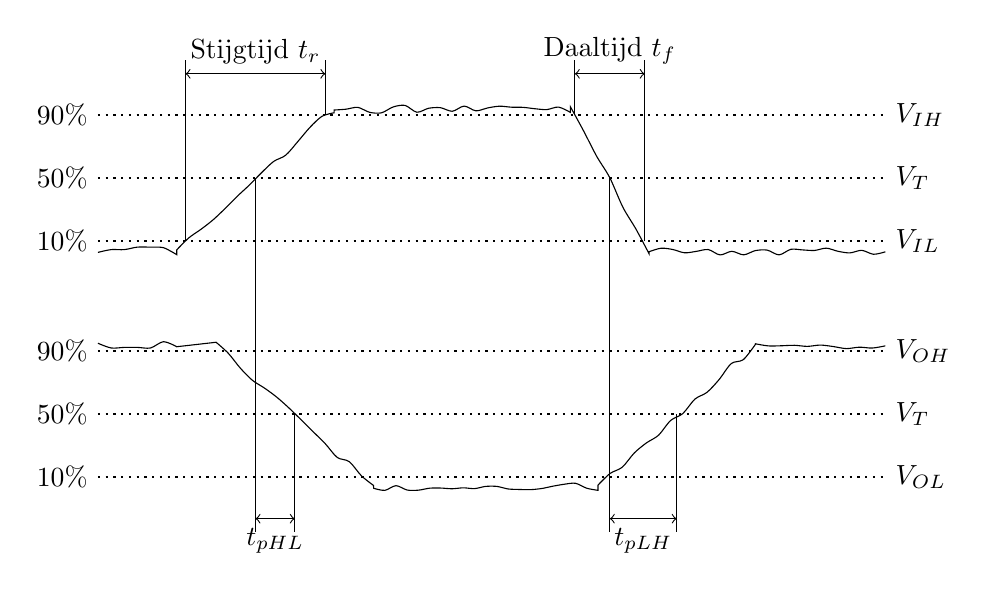
\begin{tikzpicture}
\def \yt{2.5};
\def \yts{2.325};
\def \yb{-3.5};
\def \ybs{-3.325};
\begin{scope}[yscale=2]
\draw[dotted,thick] (0,0.9) node[anchor=east]{$90\%$} -- ++(10,0) node[anchor=west]{$V_{IH}$};
\draw[dotted,thick] (0,0.5) node[anchor=east]{$50\%$} -- ++(10,0) node[anchor=west]{$V_T$};
\draw[dotted,thick] (0,0.1) node[anchor=east]{$10\%$} -- ++(10,0) node[anchor=west]{$V_{IL}$};
\draw plot[thick,samples=7,black!80,variable=\x,domain=0:1,smooth] (\x,{0.05+0.025*rand-0.0125}) -- plot[thick,samples=14,black!80,variable=\x,domain=1:3,smooth] (\x,{0.05+0.45*\x-0.45+0.025*rand-0.0125}) -- plot[thick,samples=21,black!80,variable=\x,domain=3:6,smooth] (\x,{0.95+0.025*rand-0.0125}) -- plot[thick,samples=7,black!80,variable=\x,domain=6:7,smooth] (\x,{0.95-0.9*\x+5.4+0.025*rand-0.0125}) -- plot[thick,samples=21,black!80,variable=\x,domain=7:10,smooth] (\x,{0.05+0.025*rand-0.0125});
\coordinate (IA) at (1.1111,0.1);
\coordinate (IMA) at (2,0.5);
\coordinate (IB) at (2.8889,0.9);
\coordinate (IC) at (6.0556,0.9);
\coordinate (IMB) at (6.5,0.5);
\coordinate (ID) at (6.9444,0.1);
\end{scope}
\draw (IA) -- (IA |- 0,\yt);
\draw (IB) -- (IB |- 0,\yt);
\draw (IC) -- (IC |- 0,\yt);
\draw (ID) -- (ID |- 0,\yt);
\draw[<->] (IA |- 0,\yts) to node[midway,above]{Stijgtijd $t_r$} (IB |- 0,\yts);
\draw[<->] (IC |- 0,\yts) to node[midway,above]{Daaltijd $t_f$} (ID |- 0,\yts);
\begin{scope}[yscale=2,yshift=-1.5cm]
\draw[dotted,thick] (0,0.9) node[anchor=east]{$90\%$} -- ++(10,0) node[anchor=west]{$V_{OH}$};
\draw[dotted,thick] (0,0.5) node[anchor=east]{$50\%$} -- ++(10,0) node[anchor=west]{$V_T$};
\draw[dotted,thick] (0,0.1) node[anchor=east]{$10\%$} -- ++(10,0) node[anchor=west]{$V_{OL}$};
\draw plot[thick,samples=7,black!80,variable=\x,domain=0:1,smooth] (\x,{0.95+0.025*rand-0.0125}) -- plot[thick,samples=14,black!80,variable=\x,domain=1.5:3.5,smooth] (\x,{0.95-0.45*\x+1.5*0.45+0.025*rand-0.0125}) -- plot[thick,samples=21,black!80,variable=\x,domain=3.5:6.35,smooth] (\x,{0.05+0.025*rand-0.0125}) -- plot[thick,samples=14,black!80,variable=\x,domain=6.35:8.35,smooth] (\x,{0.05+0.45*\x-0.45*6.35+0.025*rand-0.0125}) -- plot[thick,samples=11,black!80,variable=\x,domain=8.35:10,smooth] (\x,{0.95+0.025*rand-0.0125});
\coordinate (OMA) at (2.5,0.5);
\coordinate (OMB) at (7.35,0.5);
\end{scope}
\draw (IMA) -- (IMA |- 0,\yb);
\draw (OMA) -- (OMA |- 0,\yb);
\draw (IMB) -- (IMB |- 0,\yb);
\draw (OMB) -- (OMB |- 0,\yb);
\draw[<->] (IMA |- 0,\ybs) to node[midway,below]{$t_{pHL}$} (OMA |- 0,\ybs);
\draw[<->] (IMB |- 0,\ybs) to node[midway,below]{$t_{pLH}$} (OMB |- 0,\ybs);
\end{tikzpicture}
\caption{Het dynamisch gedrag van een NOT-poort.}
\figlab{dynamicBehaviorNotGate}
\end{figure}
We hebben het reeds uitvoerig gehad over het dynamisch karakter van een elektronische schakeling. Naast het feit dat het enige tijd duurt alvorens een spanning die op een draad wordt aangelegd daadwerkelijk dit spanningsniveau bereikt, heeft ook een poort een dynamisch karakter. Een interessante eigenschap is dat de stijg- en daaltijd invloed hebben op de vertraging van de poort. We zullen deze drie grootheden nu formaliseren:
\begin{itemize}
 \item \termen{Stijgtijd $t_r$} ofwel \termen{rise time}: de tijd die de spanning nodig heeft om van een lage spanning naar een hoge spanning te stijgen. Men neemt hiervoor de 10\% en 90\% grenzen tussen de basisspanning en de topspanning\footnote{In sommige publicaties wordt 80\% en 20\% gebruikt.}.
 \item \termen{Daaltijd $t_f$} ofwel \termen{fall time}: de tijd die de spanning nodig heeft om van een hoge spanning naar een lage spanning te dalen. Men neemt hiervoor de 90\% en 10\% grenzen tussen de basisspanning en de topspanning.
 \item \termen{Vertragingstijd $t_p$} ofwel \termen{propagation delay}: De tijd die de poort nodig heeft tussen de ingangspanning die het midden bereikt tussen de basisspanning en de topspanning, en de uitgang die deze 50\% grens bereikt. Vermits de stijg- en daaltijd ook bepalen hoe snel een signaal naar 50\% stijgt of daalt, hebben deze parameters ook invloed op de vertragingstijd. We berekenen de vertraging door het gemiddelde te nemen tussen de vertraging tijdens het dalen $t_{pHL}$ en het stijgen $t_{pLH}$:
\begin{equation}
\mbox{Vertragingstijd $t_p$}=\displaystyle\frac{t_{pHL}+t_{pLH}}{2}
\end{equation}
\end{itemize}
Dit principe wordt ge\"illustreerd op \figref{dynamicBehaviorNotGate}. We zien hier twee situaties: in de eerste situatie is de stijgtijd van de ingang gelijk aan de daaltijd van de uitgang. De poort heeft weliswaar een vertraging, maar deze is vrij beperkt. In het tweede geval is de stijgtijd van de uitgang dubbel zolang als de daaltijd van de ingang. Hoewel de poort sneller reageert op het veranderende signaal, is de vertraging groter. Vermits de stijg- en daaltijden be\"invloed worden door de parasitaire capaciteit\footnote{De capaciteit die wordt veroorzaakt door de draad zelf.}, wordt dus ook de vertraging be\"invloed door de aard van de draden. De vertraging bij korte draden is aanzienlijk kleiner dan deze van lange draden.
%??%TODO
%De ingangsimpedantie is hierbij omgekeerd evenredig met de \termen{Stijgtijd}. De uitgangsimpedantie is evenredig met de \termen{Daaltijd}. Deze 
\subsection{Vermogenverbruik}
Een van de belangrijkste ontwerpbeperkingen bij grote schakelingen is het \termen{vermogenverbruik}. Het vermogenverbruik is dan ook een parameter die zich negatief uit op twee verschillende domeinen:
\begin{itemize}
 \item Levering: De verbruikte energie heeft een kostprijs, bovendien uit het vermogenverbruik zich ook in een kortere levensduur van eventuele batterijen.
 \item Gedissipeerd: het vermogenverbruik leidt tot warmteontwikkeling. Deze warmte moet afgevoerd worden, wat ook vermogenverbruik met zich meebrengt.
\end{itemize}
We beschouwen twee vormen van vermogenverbruik:
\begin{itemize}
 \item \termen{Statisch vermogenverbruik}: Dit is het vermogen die continu verbruikt wordt, ook indien de schakeling niets doet. We zagen reeds dat dit bij NMOS implementaties het geval is, omdat we bij het sluiten van een NMOS-transistor, een lekstroom genereren van de source naar de drain. Bij NMOS-poorten mogen we dan ook uitgaan van een vermogenverbruik van $1\mbox{ mW}$. Dit betekent dus voor een gemiddelde chip dat dit makkelijk oploopt in tot $1\mbox{ kW}$ wat totaal onaanvaardbaar is. Bij CMOS hebben we eenvoudigweg geen lekstroom en dus ook geen statisch vermogenverbruik.
 \item \termen{Dynamisch vermogenverbruik}: Dit is het vermogen die verbruikt wordt op het moment dat een poort omschakelt. Hierdoor wordt de parasitaire capaciteit $C$ op- of ontladen. In \cite[3.12]{brown2004fundamentals} wordt hiervoor volgende formule gegeven:
\begin{equation}
P_{\mbox{\small{dyn.}}}=C\times f\times V^2
\end{equation}
Met chipoppervlakte $C$, een klokfrequentie $f$ en voedingsspanning $V$. We kunnen deze formule als volgt verklaren: Vermits het chipoppervlakte hoofdzakelijk draden bevat is dit een goede schatting voor de totale lengte van de draden, verder bepaalt de klokfrequentie hoeveel maal we per seconde deze draden moeten op- en ontladen. Het vermogen ten slotte om een capaciteit $C$ op te laden is evenredig met het kwadraat van de spanning. In de praktijk werken de meeste schakelingen met een klokfrequentie in de grootorde van $100\mbox{ MHz}$. Verder schakelen uiteraard niet alle draden telkens om, een realistische schatting ligt bij de 20\%. Indien we ook de oppervlakte van een poort in rekening brengen komen we uit op een ordegrootte van $35\mbox{ nW}$ per inverter. We kunnen dus in de grootorde van $300\ 000\ 000$ invertoren plaatsen voor een vermogenverbruik van $1\mbox{ W}$. In de praktijk is vermogenverbruik dan ook een van de belangrijkste beperkingen om rekening mee te houden bij het ontwerpen van digitale schakelingen, vandaar dat er in deze cursus ook een grote nadruk ligt op het minimaliseren van digitale schakelingen.
??%TODO%In de praktijk komt dit ongeveer overeen met $35\mbox{ nW}$ per inverter in een poort. Hierbij maken we een assumptie dat per klokcyclus, 20\% van de poorten omschakelt, en we een klokfrequentie rond de $100\mbox{ MHz}$ gebruiken.
\end{itemize}
\subsection{``1'' en ``0'' doorgeven}
Een oplettend lezer zal zich misschien de vraag gesteld hebben, waarom we een buffer zoals op \figref{bufferCmos} op pagina \pageref{fig:bufferCmos} niet implementeren door de NMOS en PMOS transistor om te wisselen. Dit zou ons immers twee transistoren besparen, en bovendien zou de poort effici\"enter werken, zoals op \figref{badBufferCmos}. Deze methode kunnen we echter niet consistent hanteren. Voor de verklaring moeten we terug naar een belangrijk detail bij de werking van transistoren in sectie \ref{ss:nmosPmosWork}. Een NMOS transistor geleidt immers alleen maar indien de spanning tussen de basis en de collector $V_{GS}$, groter is dan de transferspanning $V_{T}$. Indien de NMOS transistor dus gesloten is, zal de uitgangsspanning $V_{T}$ lager zijn dan de ingangsspanning. Dit geeft misschien bij \'e\'en transistor geen noemenswaardige problemen, maar bij een sequentie van transistoren, zal de spanning uiteindelijk onder het grensniveau vallen. Samenvattend kunnen we zeggen dat NMOS transistoren hoge spanningen niet goed doorgeven, en dus een slechte pull-up zijn. Analoog voor PMOS geldt dezelfde redenering, maar dan toegepast op lage spanningen. Een PMOS transistor is dus een slechte pull-down. Deze spanningsverschillen zijn ook gevisualiseerd op \figref{badBufferCmos}.
\begin{figure}[hbt]
\centering
\subfigure[Buffer met inverterende poorten]{\begin{tikzpicture}[circuit logic US]
\coordinate (F0) at (-3,0);
\coordinate (I) at (-2,0);
\draw (F0) node[anchor=east,scale=0.75]{$x$} -- (I);
\node [pmoso] (P1) at (-1,0.75) {};
\draw (I) |- (P1.gate);
\draw[->] (P1.source) -- ++(0,0.5) node[anchor=west,scale=0.75]{$V_{\mbox{\tiny DD}}$};
\node [nmosc] (N1) at (-1,-0.75) {};
\draw (I) |- (N1.gate);
\draw (N1.source) node [ground] {};
\draw (N1.drain) -- (P1.drain);
\node [pmosc] (P2) at (1,0.75) {};
\coordinate (F1) at (-1,0);
\coordinate (O) at (0,0);
\draw (F1) -- (O);
\draw[->] (P2.source) -- ++(0,0.5) node[anchor=west,scale=0.75]{$V_{\mbox{\tiny DD}}$};
\draw (O) |- (P2.gate);
\node [nmoso] (N2) at (1,-0.75) {};
\draw (O) |- (N2.gate);
\draw (N2.source) node [ground] {};
\draw (N2.drain) -- (P2.drain);
\coordinate (F2) at (1,0);
\draw (F2) -- ++(1,0) node[anchor=west,scale=0.75]{$f$};
\end{tikzpicture}
\figlab{goodBufferCmos}
}
\subfigure[Fout buffer]{\begin{tikzpicture}[circuit logic US]
\coordinate (F0) at (-3,0);
\coordinate (I) at (-2,0);
\draw (F0) node[anchor=east,scale=0.75]{$x$} -- (I);
\node [nmosc] (N1) at (-1,0.75) {};
\draw (I) |- (N1.gate);
\draw[->] (N1.drain) -- ++(0,0.5) node[anchor=west,scale=0.75]{$V_{\mbox{\tiny DD}}$};
\node [pmoso] (P1) at (-1,-0.75) {};
\draw (I) |- (P1.gate);
\draw (P1.drain) node [ground] {};
\draw (P1.source) -- (N1.source);
\coordinate (F1) at (-1,0);
\coordinate (O) at (0,0);
\draw[->,black!80,dashed] (-1.625,0 |- N1.gate) arc (180:270:0.625);
\draw[black!80] (-0.625*0.607-1,0.75-0.625*0.607) node[scale=0.75,anchor=north east]{$V_T$};
\draw (F1) -- (O) node[anchor=west,scale=0.75]{$f$};
\end{tikzpicture}
\figlab{badBufferCmos}
}
\caption{Buffer ge\"implementeerd met omgekeerde transistoren: NMOS is een slechte pull-up.??}%TODO: betere naam zoeken.
\figlab{badNmosPmos}
\end{figure}
\subsection{Fan-in en fan-out}
Enkele belangrijke eigenschappen van een poort zijn de \termen{fan-in} en \termen{fan-out}. De fan-in is het aantal ingangen die de poort in kwestie heeft. Deze eigenschap is eigen aan het type poort\footnote{Bijvoorbeeld een 3-nand heeft een fan-in van 3.}. De fan-out is het aantal ingangen van andere poorten die de poort kan aansturen, het aantal draden die uit de poort in kwestie komt zeg maar. Deze eigenschappen bepalen in grote mate de vertraging van een circuit. Indien we immers een groot aantal ingangen hebben, kan het een tijdje duren vooraleer de stroom doorheen de transistoren van de andere ingangen stroomt, als \'e\'en van de transistoren omschakelt. Verder zullen we ook de spanning moeten opdrijven bij een groot aantal transistoren die we in serie schakelen. Elke transistor heeft immers indien gesloten nog steeds een kleine weerstand. Indien de stroom door een serie transistoren moet vloeien, betekent dit dat de uitgangsspanning van de poort teveel gereduceerd zou zijn. Een hogere spanning leidt weer tot hogere vermogens wat we juist willen tegengaan. Bijgevolg willen we de fan-in zo laag mogelijk houden. Daarom komen in de realiteit poorten met een groot\footnote{Met groot bedoelen we meer dan 5 ingangen.} aantal ingangen nooit voor, indien men een poort met een groot aantal ingangen wil realiseren zal men deze meestal met een sequentie van eenvoudige poorten realiseren. Ook de fan-out moeten we onder controle houden. Elke poort heeft immers maar \'e\'en uitgang. Door deze uitgang moet alle stroom naar de ingangen van andere poorten stromen. Vermits de stroom over een draad beperkt is, kunnen we spreken over een \termen{maximale stroomsterkte $I_{\mbox{\small{Omax}}}$}. Deze stroomsterkte bepaalt dan weer hoe snel we de parasitaire capaciteit kunnen op- en ontladen:
\begin{equation}
I_{\mbox{\small{Omax}}}=C\cdot\displaystyle\frac{\partial V}{\partial t}
\end{equation}
Vermits de snelheid waarmee deze capaciteit op- en ontlaadt op zijn beurt weer invloed heeft op de vertraging, heeft het ook invloed op de \termen{maximale frequentie $f_{\mbox{\small{max}}}$} van de elektronische schakeling:
\begin{equation}
f_{\mbox{\small{max}}}=\displaystyle\frac{1}{\Delta V}\cdot\displaystyle\frac{\partial V}{\partial t}=\displaystyle\frac{I_{\mbox{\small{Omax}}}}{C\cdot \Delta V}
\end{equation}
Verder zal ook de parasitaire capaciteit zelf toenemen: de uitgang die met alle ingangen verbonden is vormt \'e\'en draad. Vermits de grootte van deze draad zal afhangen van de fan-out zal dus ook de parasitaire capaciteit toenemen. We kunnen de fan-out beperken door gebruik te maken van buffers: we verdelen de uitgang van de poort onder een paar buffers die op hun beurt de ingangen van de andere poorten bevoorraden. Het nadeel van het gebruik van een buffer is dat dit buffer ook moet omschakelen, wat extra vermogenverbruik en vertragingen teweeg brengt.
\subsection{Tri-state buffer}
Een uitbreiding van een buffer is een \termen{Tri-state buffer} ofwel \termen{3-state buffer}. \figref{triStateSymbol} toont het symbool die men voor deze component gebruikt: een buffer met een derde ingang aan de zijkant van de driehoek. Een tri-state buffer heeft drie mogelijke uitgangswaarden: 0, 1 en de zogenaamde \termen{zwevende modus $Z$}. Deze laatste toestand wordt ook wel \termen{hoog impedant} genoemd. Het betekent dat de lijn losgekoppeld is van enige bron. Er staat dus zogezegd niets op de lijn. Hiertoe wordt een buffer uitgebreid met een tweede ingang: \termen{Enable $E$}. Hierdoor kan de component in drie toestanden worden gebracht: wanneer enable op 0 staat, staat de tri-state buffer in de $Z$ stand. In het geval er een hoog signaal op de enable-ingang wordt aangelegd, laat het de ingang door, deze kan uiteraard in twee standen staan. Op \figref{triStateTruth} wordt dit concept met behulp van een waarheidstabel weergegeven. Er bestaan verschillende manieren om deze component te implementeren. Een goedkope manier wordt voorgesteld op \figref{triStateImplementation} en maakt gebruik van een \termen{transmission gate}, een component die functioneert als een schakelaar.
\begin{figure}[hbt]
\centering
\subfigure[Symbool]{
\begin{tikzpicture}
\node[tris] (TS) at (0,0) {};
\draw (TS.c) -- ++(0,-0.5) node[anchor=north]{enable $e$};
\draw (TS.x) -- ++(-0.5,0) node[anchor=east]{input $x$};
\draw (TS.z) -- ++(0.5,0) node[anchor=west]{output $f$};
\end{tikzpicture}
\figlab{triStateSymbol}}
\subfigure[Tabel]{
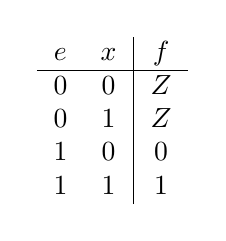
\begin{tikzpicture}
\node (A) at (0,0) {\begin{tabular}{cc|c}
$e$&$x$&$f$\\\hline
$0$&$0$&$Z$\\
$0$&$1$&$Z$\\
$1$&$0$&$0$\\
$1$&$1$&$1$
\end{tabular}};
\end{tikzpicture}
\figlab{triStateTruth}}
\subfigure[Implementatie]{
\begin{tikzpicture}[circuit logic US]
\node[transgate] (TG) at (0,0) {};
\node[not gate,scale=0.8] (N1) at (-1,0) {};
\node[not gate,scale=0.8] (N2) at (-2,0) {};
\node[not gate,scale=0.8] (N3) at (-1,1) {};
\draw (N1.output) -- (TG.x);
\draw (N2.output) -- (N1.input);
\draw (N2.input) -- (-3,0 |- N2.input) node[anchor=east]{$x$};
\draw (N3.input) -- (-3,0 |- N3.input) node[anchor=east]{$e$};
\draw (N3.output) -| (TG.cn);
\draw (TG.z) -- ++(0.5,0) node[anchor=west]{$f$};
\pdot{-2.6,1};
\draw (-2.6,1) |- (0,-1) -- (TG.c);
\end{tikzpicture}
\figlab{triStateImplementation}}
\subfigure[Transmission Gate]{
\begin{tikzpicture}
\node[transgate] (TG) at (0,0) {};
\draw (TG.x) -- ++(-0.5,0) node[anchor=east]{$x$};
\draw (TG.z) -- ++(0.5,0) node[anchor=west]{$f$};
\draw (TG.cn) -- ++(0,0.5) node[anchor=south]{$\bar{s}$};
\draw (TG.c) -- ++(0,-0.5) node[anchor=north]{$s$};
\draw (1.75,0) node{$\equiv$};
\begin{scope}[xshift=4 cm]
\node[pmosc,rotate=-90] (P) at (0,0.5) {};
\node[nmosc,rotate=90] (N) at (0,-0.5) {};
\coordinate (X) at (-0.75,0);
\coordinate (F) at (0.75,0);
\draw (P.source) -| (F) |- (N.source);
\draw (P.drain) -| (X) |- (N.drain);
\draw (X) -- ++(-0.5,0) node[anchor=east]{$x$};
\draw (F) -- ++(0.5,0) node[anchor=west]{$f$};
\draw (P.gate) -- ++(0,0.5) node[anchor=south]{$\bar{s}$};
\draw (N.gate) -- ++(0,-0.5) node[anchor=north]{$s$};
\pdot{X};\pdot{F};
\end{scope}
\end{tikzpicture}
\figlab{triStateTransmission}}
\subfigure[Bus]{
\begin{tikzpicture}[circuit logic US]
\node[tris] (T1) at (-0.75,0.5) {};
\node[tris] (T2) at (-0.75,-0.5) {};
\node[buffer gate] (B1) at (0.75,1) {};
\node[buffer gate] (B2) at (0.75,0) {};
\node[buffer gate] (B3) at (0.75,-1) {};
\draw (B1.input) -| (0,0) |- (B3.input);
\draw (0,0) -- (B2.input);\draw (0,0.5) -- (T1.z);\draw (0,-0.5) -- (T2.z);
\draw (T1.x) -- (T1.x -| -1.5,0) node[anchor=east]{$x_1$};
\draw (T1.c) |- (-1.25,0) node[anchor=east]{$e_1$};
\draw (T2.x) -- (T2.x -| -1.5,0) node[anchor=east]{$x_2$};
\draw (T2.c) |- (-1.25,-1) node[anchor=east]{$e_2$};
\draw (B1.output) -- ++(0.5,0) node[anchor=west]{$f_1$};
\draw (B2.output) -- ++(0.5,0) node[anchor=west]{$f_2$};
\draw (B3.output) -- ++(0.5,0) node[anchor=west]{$f_3$};
\pdot{0,0};\pdot{0,-0.5};\pdot{0,0.5};
\end{tikzpicture}
\figlab{triStateBus}}
\caption{Tri-state buffer.}
\end{figure}
De transmission gate zelf bestaat zoals te zien op \figref{triStateTransmission} uit twee transistoren. Indien $s=0$ zijn beide schakelaars open, en staat er dus geen signaal op uitgang $f$, in dat geval is de uitgang dus hoog impedant. Bij $s=1$ zijn beide transistoren gesloten, en wordt het signaal die aangelegd wordt op $x$ verder gepropageerd. De schakeling op \ref{fig:triStateImplementation} bevat extra componenten om het binnenkomende signaal opnieuw voldoende sterk te maken, dezelfde argumenten als met fan-in en fan-out gelden hier immers.
\paragraph{Bus}Tri-state buffers worden vaak gebruikt om bijvoorbeeld over een lijn gegevens van verschillende bronnen over te brengen. We hebben reeds in \ref{term:kortsluiting} gezien dat het verbinden van uitgangen tot kortsluiting leidt. Hierdoor zouden we echter genoodzaakt zijn om voor elke uitgang een aparte draad te voorzien. Verbindingen kunnen een groot gedeelte van het chipoppervlak beslaan, vandaar dat we het aantal draden ook tot een minimum proberen te beperken. We kunnen dit probleem oplossen met een zogenaamde \termen{bus}. Bij een bus wordt een draad gedeeld tussen verschillende bronnen $x_i$. Elk van die bronnen stuurt een tri-state buffer aan. Verder zorgt men er voor dat er slechts \'e\'en tri-state buffer tegelijk actief is. Omdat de andere tri-state buffers op dat moment hoog-impedant zijn, is er geen gevaar voor kortsluiting. \figref{triStateBus} geeft een implementatie van dit principe. In subsectie \ref{ss:multiplexer} zullen we verder een component tegenkomen die dit principe met een algemenere techniek realiseert: de multiplexer. In dat geval moeten de andere bronnen een $Z$ op de lijn zetten.
% \section{CAD-ontwerp in de praktijk}
% \subsection{Ingave}
% \subsection{Synthese}
% \subsection{Fysisch}
% \subsection{Chip}
%TODO: cad
